\documentclass{article}

\usepackage{iclr2026_conference,times}
\usepackage{graphicx}
\usepackage{booktabs}
\usepackage{array}
\usepackage{amsmath}
\usepackage{amssymb}
\usepackage{amsthm}
\usepackage{enumitem}
\usepackage{url}

\title{Action Aliasing in Robot Foundation Models}

\author{Anonymous Authors}

\newtheorem{definition}{Definition}
\newtheorem{proposition}{Proposition}
\newtheorem{assumption}{Assumption}
\newtheorem{corollary}{Corollary}

\newcommand{\A}{\mathcal{A}}
\newcommand{\Sspace}{\mathcal{S}}
\newcommand{\Z}{\mathcal{Z}}
\newcommand{\E}{\mathcal{E}}
\newcommand{\Obs}{\mathcal{O}}
\newcommand{\diam}{\operatorname{diam}}
\newcommand{\EE}{\mathbb{E}}

\begin{document}

\maketitle

\begin{abstract}
Robot foundation models increasingly expose robot control through language-like
or discretized action tokens. This interface is convenient for sequence
modeling, but it can be physically non-identifiable: one token may denote a
fiber of low-level commands whose members produce different next-state effects
under local robot dynamics. We formalize this failure as \emph{action aliasing}.
The central diagnostic is the effect diameter of a token fiber, not token
accuracy, raw action distance, or language similarity. A simple lower bound
shows that any decoder observing only a token must incur worst-case one-step
effect error at least half the token fiber's effect diameter. We then introduce
Effect-Separating Action Charts (ESAC), an audit-and-repair layer that splits
aliased token fibers by observed transition effects and trains a chart predictor
to decode the appropriate local action chart. The final evidence is a synthetic
but full-scale mechanism study with nine suites, 2,526 compact metric rows, and
2,005,200 evaluated predictions counted across rows. At alias strength 1.25 in
the main suite, coarse token decoding reaches 0.140 success, raw action charts
0.605, ESAC with hidden alias context 0.356, ESAC with full alias context 0.728,
continuous regression upper 0.998, and oracle replay 1.000. Boundary controls
are equally important: oracle mode/contact tokenization raises coarse-token
success to 0.760, a single-token alias control collapses ESAC to 0.032, and ESAC
falls to 0.356 when alias-resolving context is hidden. The claim is therefore
narrow: action-token interfaces need physical effect audits whenever many-to-one
tokenization collapses commands whose effects matter for control. This paper
does not claim real-robot deployment or superiority over policies that bypass
the token bottleneck.
\end{abstract}

\section{Introduction}

Robot foundation models (RFMs) and vision-language-action (VLA) policies have
made it plausible to treat control as another sequence modeling problem. Images,
language, proprioception, and interaction history enter a large model, and robot
behavior leaves as a token, action chunk, or continuous action head
\citep{brohan2023rt1,brohan2023rt2,openx2023rtx,kim2024openvla,octo2024,black2024pi0}.
This abstraction is powerful. It lets robot data be mixed across embodiments,
lets language-conditioned policies reuse sequence-modeling infrastructure, and
lets actions be compressed into finite vocabularies. It also creates a quiet
failure mode. A token can be correct as a symbol while being wrong as a physical
command.

The failure is not merely calibration error or aleatoric uncertainty. It is an
identity problem. If a token interface maps several low-level commands to one
symbol, the token no longer identifies which member of that fiber should be
executed. When all members of the fiber have nearly the same effect, the
collapse is harmless. When members produce different contact transitions,
object motions, force modes, or recovery outcomes, the collapse is physically
aliased. A downstream decoder that observes only the token must choose one
effect for the whole fiber.

This paper studies that failure and a minimal repair. We define an action token
as a fiber of low-level commands and measure the fiber's \emph{effect diameter}:
the largest task-relevant next-state effect distance between commands sharing
the same token. We prove a simple lower bound showing that token-only decoding
has irreducible worst-case effect error when this diameter is large. We then
introduce Effect-Separating Action Charts (ESAC). ESAC audits each token by
effect diameter and splits aliased token fibers by observed transition effects,
not by raw motor distance or language labels.

The point is not that clustering is new. It is not. The point is where the
equivalence relation should live. Raw motor vectors can differ by nullspace
motion while producing the same object effect. Conversely, nearby motor vectors
can cause different effects in contact. ESAC therefore treats two actions as
distinct only when their next-state effects differ under the task metric.

The final evidence is intentionally synthetic but no longer narrow. We run nine
full-scale suites: main alias-strength sweeps, context-reliability stress,
token-granularity controls, chart-count ablations, data-scale sweeps,
alias-strength shift, effect-metric sensitivity, success-threshold sensitivity,
and negative controls. The suites produce 2,526 compact metric rows and
2,005,200 evaluated predictions counted across rows. The result is not a claim
that ESAC is a deployed robot system. It is a mechanism claim: if the action
interface collapses commands whose effects differ, the token is not physically
atomic and should be audited as a fiber.

\paragraph{Contributions.}
\begin{itemize}[leftmargin=1.4em]
    \item We formalize action-token aliasing through token fibers and
    task-relevant effect diameter.
    \item We prove an irreducible error lower bound for token-only decoders.
    \item We propose ESAC, which splits aliased token fibers by transition
    effects and learns a chart predictor for decoding.
    \item We report a full-scale synthetic study with positives, boundary
    controls, negative controls, noise/context stress, and metric sensitivity.
    \item We state the boundary clearly: ESAC requires observable
    alias-resolving context and a meaningful effect metric; continuous policies
    can avoid this exact bottleneck when they bypass many-to-one tokenization.
\end{itemize}

\section{Related Work}

\paragraph{Robot foundation models and VLA policies.}
RT-1 and RT-2 showed that transformer policies can map large-scale robot data
and web-scale vision-language knowledge into robot actions
\citep{brohan2023rt1,brohan2023rt2}. Open X-Embodiment and RT-X expanded this
premise across embodiments \citep{openx2023rtx}; Octo and OpenVLA made
generalist policies and VLA models more accessible
\citep{octo2024,kim2024openvla}; $\pi_0$ uses a flow model for general robot
control \citep{black2024pi0}. Survey work now treats VLA policies as a central
embodied manipulation paradigm \citep{li2025surveyvla,din2025systematic}. These
works make broad robot-data scaling, VLA grounding, and large policy training
clearly prior art. Our question is narrower: does the emitted action interface
preserve the physical distinctions needed by control?

\paragraph{Action tokenization and action representations.}
Recent work explicitly studies action tokens for VLAs, including FAST
\citep{pertsch2025fast}, keypoint action tokens
\citep{dipalo2024keypoint}, discrete policies for multi-task manipulation
\citep{wu2025discrete}, and hybrid discrete-continuous action spaces for
assembly \citep{zhang2022hybrid}. Action chunking and ACT-style policies
represent temporally extended commands \citep{zhao2023act}, while behavior
transformers model multimodal actions \citep{shafiullah2022behavior}. These
methods improve action parameterization. ESAC is different in its criterion:
two actions should be separated if their effects differ under local dynamics,
even if their language label, token id, or raw action cluster is the same.

\paragraph{Continuous visuomotor policies.}
Diffusion and flow policies can model multimodal continuous action
distributions without committing to a single discrete token
\citep{chi2024diffusion,black2024pi0}. They are important alternatives and
upper baselines, not straw men. Our theorem targets architectures, APIs, or
deployment layers that do use a many-to-one token interface. Continuous heads
can still inherit aliasing if an upstream representation has already erased the
physical distinction, but they can also bypass the exact token bottleneck.

\paragraph{Language grounding, affordances, and contact.}
VIMA, PaLM-E, SayCan, RoboCat, and related language-conditioned robot systems
connect instructions or multimodal prompts to actions and skills
\citep{jiang2022vima,driess2023palme,ahn2022saycan,bousmalis2023robocat}.
Contact-rich robotics has long shown that small differences in force,
compliance, and contact mode can change outcomes \citep{koval2015contact}.
Action aliasing is where these two facts meet: a semantic action name or token
can be too coarse for the physical distinctions that contact makes decisive.

\paragraph{Novelty boundary.}
The repository contains a 3,106-entry literature matrix, a 300-paper serious
skim, a 250-paper extraction table, and a 100-paper hostile prior-work set. The
closest hostile areas are VLA scaling, action tokenization, action chunking,
diffusion/flow actions, language-conditioned robot planning, and contact-rich
manipulation. The paper's boundary is therefore not ``new tokenization'' or
``new clustering.'' The boundary is the action-fiber/effect-diameter diagnosis
and the claim that token repair should be driven by next-state effects.

\section{Problem Setup}

Let $s\in\Sspace$ be a robot/environment state and $a\in\A$ a low-level motor
command. Let $f(s,a)$ denote one-step dynamics. The robot's task does not need
the full next state; it needs a physical effect relevant to the current control
decision. We write
\[
    \E_s(a)=\phi(f(s,a))-\phi(s),
\]
where $\phi$ maps a state to a task-relevant effect representation such as
object displacement, contact wrench change, contact-mode transition, grasp
stability feature, or a learned effect embedding. The effect space has metric
$d_\E$.

An action-token interface is a map
\[
    q_s:\A\rightarrow\Z .
\]
The state dependence allows tokenizers that include embodiment, controller
mode, or known contact context, although many interfaces are closer to a global
$q(a)$. A VLA model may output $z\in\Z$ directly, may output an action chunk
whose coarse index is a token, or may expose a skill label that later decodes
to low-level control. The analysis applies whenever several low-level commands
share one emitted symbol or interface action.

\begin{definition}[Token fiber]
For state $s$ and token $z$, the action fiber is
\[
    F_s(z)=\{a\in\A:q_s(a)=z\}.
\]
\end{definition}

\begin{definition}[Effect diameter]
The effect diameter of token $z$ at state $s$ is
\[
    \Delta_s(z)=
    \sup_{a,a'\in F_s(z)}
    d_\E\bigl(\E_s(a),\E_s(a')\bigr).
\]
\end{definition}

\begin{definition}[Action aliasing]
For task tolerance $\epsilon$, a token is $\epsilon$-aliased at state $s$ when
$\Delta_s(z)>\epsilon$.
\end{definition}

This definition deliberately ignores raw motor distance. Two motor commands can
be far apart but equivalent because their difference lies in a nullspace. Two
commands can also be close in motor space but divergent in contact. The
identity condition is effect equivalence, not vector closeness.

\begin{assumption}[Task-relevant effect metric]
The effect metric $d_\E$ is chosen so that small effect error implies acceptable
one-step task error for the local decision. This may be an engineered contact
metric, a task-space displacement metric, or a validated learned effect
embedding.
\end{assumption}

The assumption is a real limitation. If $\phi$ ignores the variable that causes
failure, then an effect-diameter audit can certify the wrong equivalence class.
The full-scale study includes metric-misspecification controls for this reason.

\section{Token-Fiber Lower Bound}

The lower bound is elementary but important. It says that once a many-to-one
token interface has collapsed effects, no token-only decoder can recover them.

\begin{proposition}[Irreducible token-fiber error]
Fix $s$ and $z$. Any decoder that observes only $z$ and predicts a single
effect $\hat e(z)$ has worst-case error
\[
    \sup_{a\in F_s(z)} d_\E(\E_s(a),\hat e(z))
    \geq \frac{1}{2}\Delta_s(z).
\]
If two actions in the fiber have Euclidean effects separated by $\Delta_s(z)$
and are equally likely, the minimum expected squared effect error is at least
$\Delta_s(z)^2/4$.
\end{proposition}

\begin{proof}
Choose $a,a'\in F_s(z)$ with effect distance arbitrarily close to
$\Delta_s(z)$. By the triangle inequality,
\[
    d_\E(\E_s(a),\E_s(a'))
    \leq d_\E(\E_s(a),\hat e)+d_\E(\hat e,\E_s(a')).
\]
At least one term is at least half their separation. Taking the supremum gives
the first claim. In Euclidean effect space, the best single prediction for two
equiprobable endpoints is their midpoint, yielding squared error
$(\Delta_s(z)/2)^2$ for both endpoints.
\end{proof}

\begin{corollary}[Token accuracy is insufficient]
High token prediction accuracy does not certify physical control accuracy when
the predicted token has large effect diameter.
\end{corollary}

The corollary matters for evaluation. A robot policy can predict the same token
as a demonstration while still lacking the information needed to choose the
right member of the fiber. Conversely, a continuous policy that bypasses the
fiber can avoid this lower bound. That is why the continuous regression baseline
in the experiments is treated as an upper comparator rather than as a method
ESAC should beat.

\section{Effect-Separating Action Charts}

ESAC is an audit-and-repair layer for tokenized robot policies. Given
transitions $(s_i,o_i,a_i,s'_i,z_i)$, compute task-relevant effects
\[
    e_i=\phi(s'_i)-\phi(s_i).
\]
For each token $z$, collect $I_z=\{i:z_i=z\}$ and estimate a within-fiber
effect radius,
\[
    \widehat R(z)=
    \left(\frac{1}{|I_z|}\sum_{i\in I_z}
    \|e_i-\bar e_z\|_2^2\right)^{1/2}.
\]
Tokens with small $\widehat R(z)$ are left alone. Tokens with large
$\widehat R(z)$ are split into charts by clustering or covering the effects
$\{e_i:i\in I_z\}$. A chart predictor $h(o_i,z_i)$ maps observations and tokens
to chart ids. A chart decoder then emits a prototype action or a local
continuous decoder for $(z,k)$.

\begin{enumerate}[leftmargin=1.4em]
    \item Log transitions with emitted token, low-level action, observation,
    and next state.
    \item Choose the effect map $\phi$ for the task.
    \item Estimate effect radius or effect diameter inside each token fiber.
    \item Flag aliased tokens whose effect radius exceeds tolerance.
    \item Split flagged fibers in effect space.
    \item Train a chart predictor from observation and token to chart id.
    \item Decode through the selected chart.
    \item Re-audit residual chart effect radius.
\end{enumerate}

The design choice is the clustering space. ESAC clusters within a token by
transition effect, not by raw motor command. This matters for redundant robots:
many motor vectors may be nullspace-equivalent, while nearby vectors can have
different object effects under contact.

\section{Synthetic Contact-Control Environment}

\paragraph{State and action.}
The simulator is deliberately small. It isolates action aliasing without
claiming realism. The state includes a command angle $\theta$, a binary mode,
a binary contact sign, friction, embodiment index, and clearance. The low-level
motor command $a\in\mathbb{R}^4$ contains planar command channels and two hidden
wrist/force channels. Local dynamics are linear in the action,
\[
    e = B(s)a,
\]
where $e\in\mathbb{R}^2$ is the object effect. The dynamics matrix depends on
contact, mode, friction, embodiment, and an alias-strength parameter.

\paragraph{Tokenization.}
The default action token keeps only an eight-way cardinal label derived from
$\theta$. It discards the mode/contact variables that make hidden wrist/force
channels physically different. Two demonstrations can therefore share one token
while requiring different effects. We also add motor nullspace variation:
different low-level commands can produce the same object effect. This makes raw
action clustering a nontrivial baseline, because it may split nuisance motor
variation rather than effect variation.

\paragraph{Methods.}
The main comparison includes:
\begin{itemize}[leftmargin=1.4em]
    \item \textbf{Coarse token}: one action prototype per token.
    \item \textbf{Raw action charts}: split each token by raw motor-command
    clusters.
    \item \textbf{ESAC, hidden context}: split by effect, but hide
    alias-resolving mode/contact variables from the chart predictor.
    \item \textbf{ESAC, full context}: split by effect with mode/contact
    visible.
    \item \textbf{Continuous regression upper}: a continuous-action regressor
    that bypasses token repair.
    \item \textbf{Oracle expert}: replay the expert command.
\end{itemize}

\paragraph{Scale.}
The final full-scale artifact has nine suites and 2,526 compact metric rows.
The main alias sweep and context-reliability sweep use 10 seeds with 2,600
training transitions and 1,000 test transitions per default condition. The
breadth suites use 8 seeds with 1,600 training transitions and 700 test
transitions, except data-scale rows that sweep 500, 1,000, 2,000, and 4,000
training transitions. Counting each row's test predictions, the artifact
contains 2,005,200 evaluated predictions. Raw train/test arrays are not stored.

\section{Full-Scale Results}

\begin{figure}[t]
    \centering
    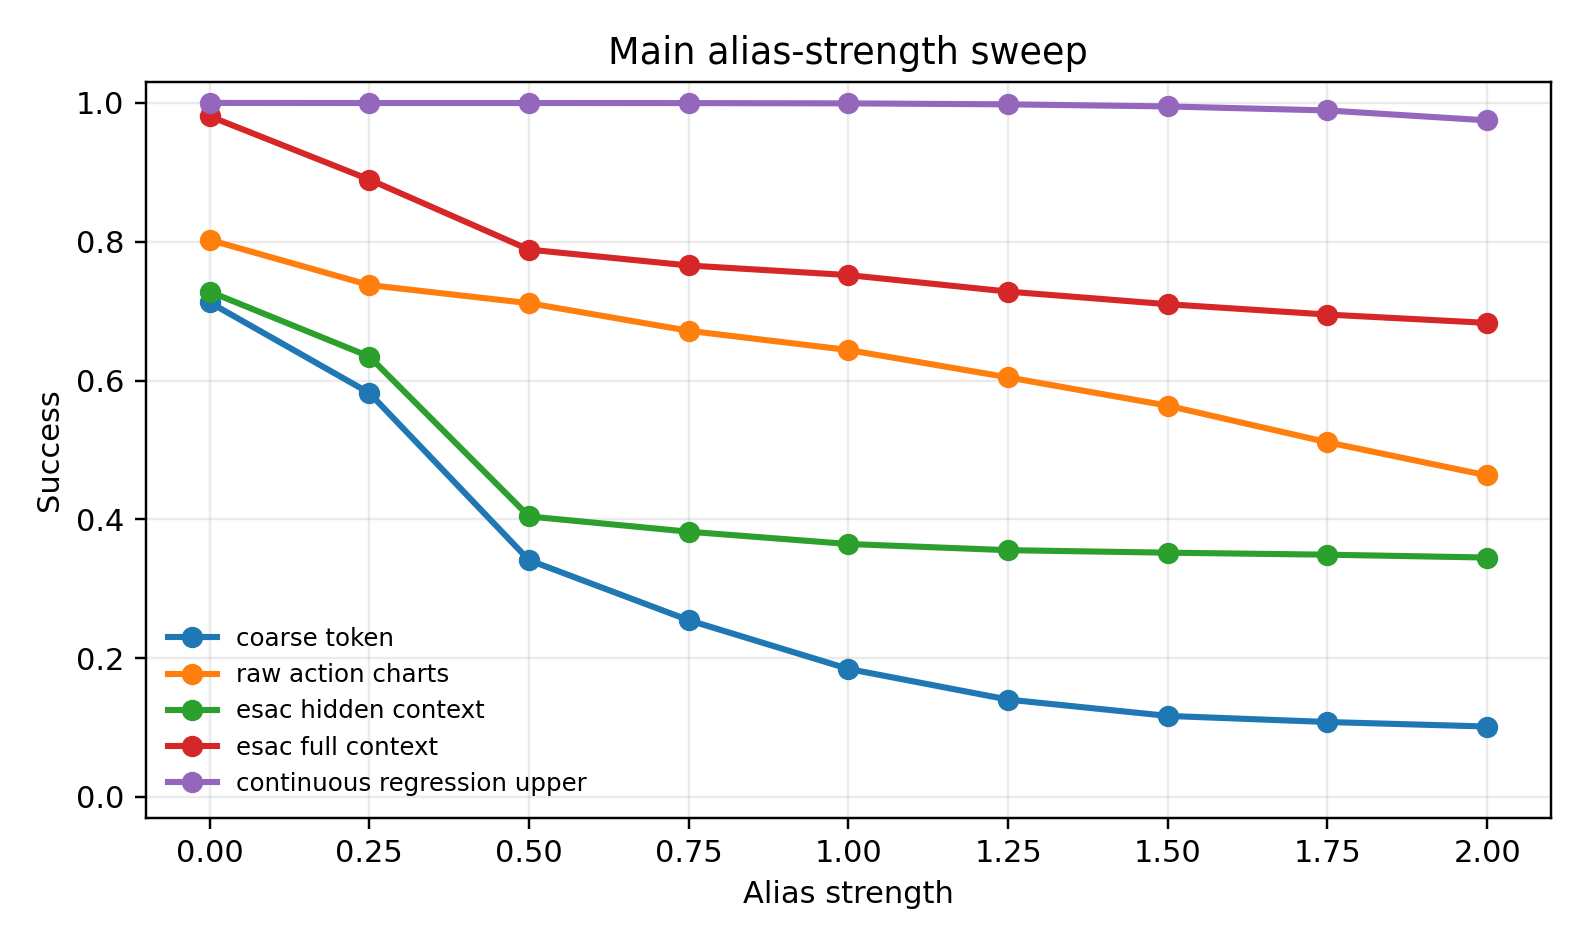
\includegraphics[width=0.49\linewidth]{figures/main_alias_sweep.png}
    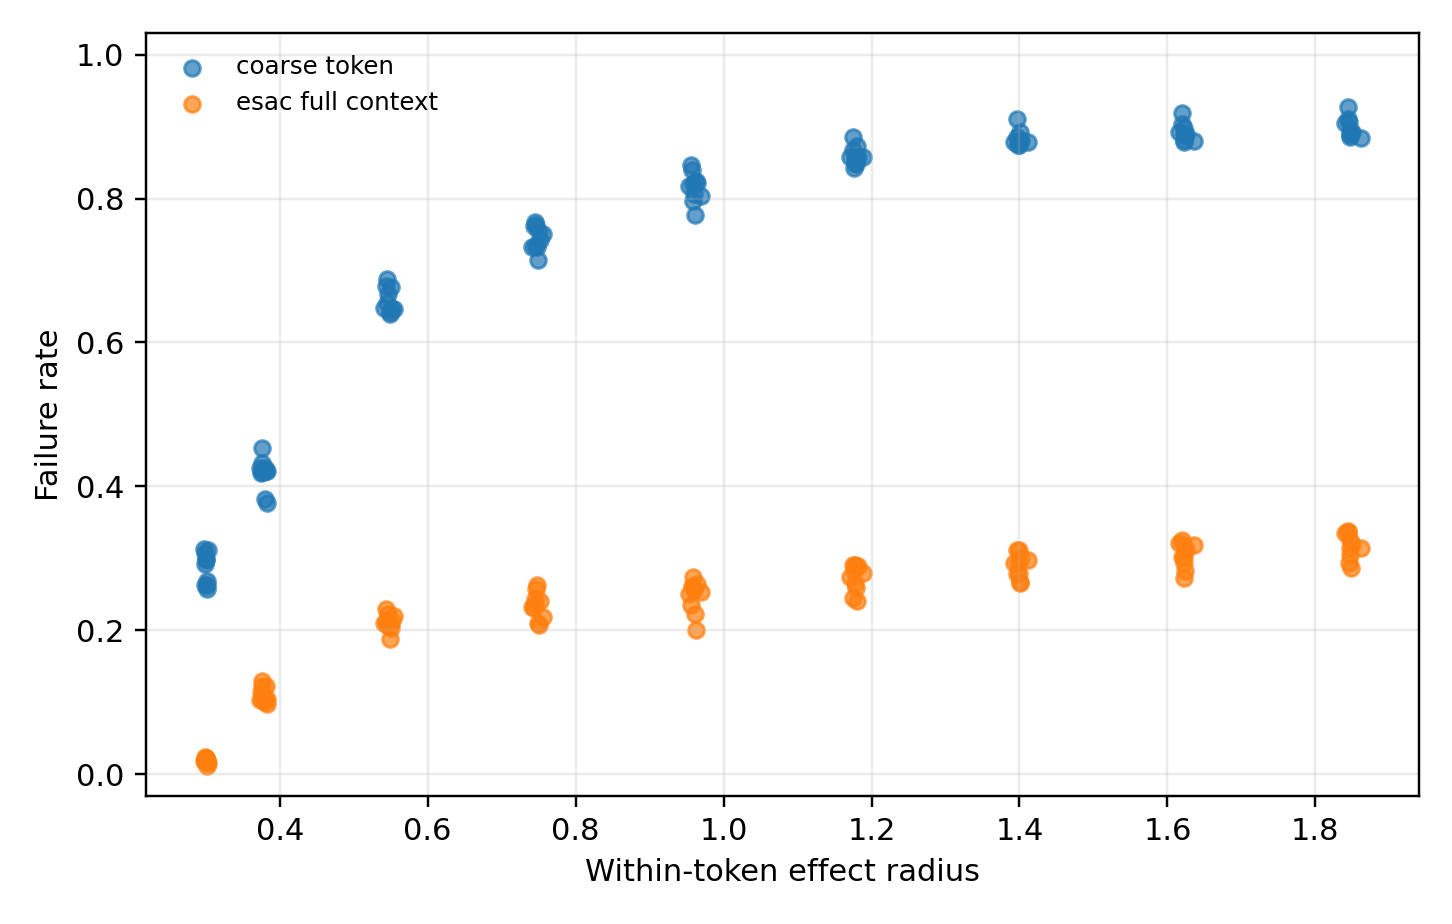
\includegraphics[width=0.49\linewidth]{figures/alias_energy_diagnostic.png}
    \caption{Left: success across alias strength. Coarse token decoding fails
    as within-token effects separate. ESAC remains useful when alias-resolving
    context is observable. Right: within-token effect radius is a direct
    diagnostic for coarse-token failure.}
    \label{fig:main}
\end{figure}

\begin{table}[t]
\centering
\caption{Main full-scale readout at alias strength $1.25$, averaged over 10
seeds. Success means one-step effect error below $0.36$.}
\label{tab:main}
\resizebox{\linewidth}{!}{
\begin{tabular}{lccc}
\toprule
Method & Success & Interpretation & Boundary \\
\midrule
Coarse token & 0.140 & One prototype per token cannot separate the fiber & Token bottleneck \\
Raw action charts & 0.605 & Motor clusters help but chase nullspace variation & Better than token, weaker than effect charts \\
ESAC, hidden context & 0.356 & Effect charts without chart-identifying observations & Fails when alias variables are unavailable \\
ESAC, full context & 0.728 & Effect charts plus observable mode/contact context & Main repair \\
Continuous regression upper & 0.998 & Bypasses many-to-one token repair & Not a token method \\
Oracle expert & 1.000 & Replays expert command & Upper bound \\
\bottomrule
\end{tabular}}
\end{table}

Table~\ref{tab:main} is the core result. The gap between coarse token decoding
and ESAC is large: 0.140 versus 0.728 success. The raw-action-chart baseline is
also informative. It reaches 0.605, showing that splitting a token helps, but
it remains below ESAC because the motor command contains nullspace variation.
The hidden-context ablation reaches only 0.356, showing that ESAC is not an
oracle. It needs observations that identify which chart applies.

The main sweep adds the shape of the effect. At alias strength 0.0, coarse
tokens already reach 0.713 and ESAC reaches 0.981. At alias strength 2.0,
coarse tokens fall to 0.102 while ESAC remains at 0.683. This pattern supports
the mechanism: the harder the token fiber separates physically, the worse a
single prototype becomes.

\subsection{Context Reliability}

\begin{figure}[t]
    \centering
    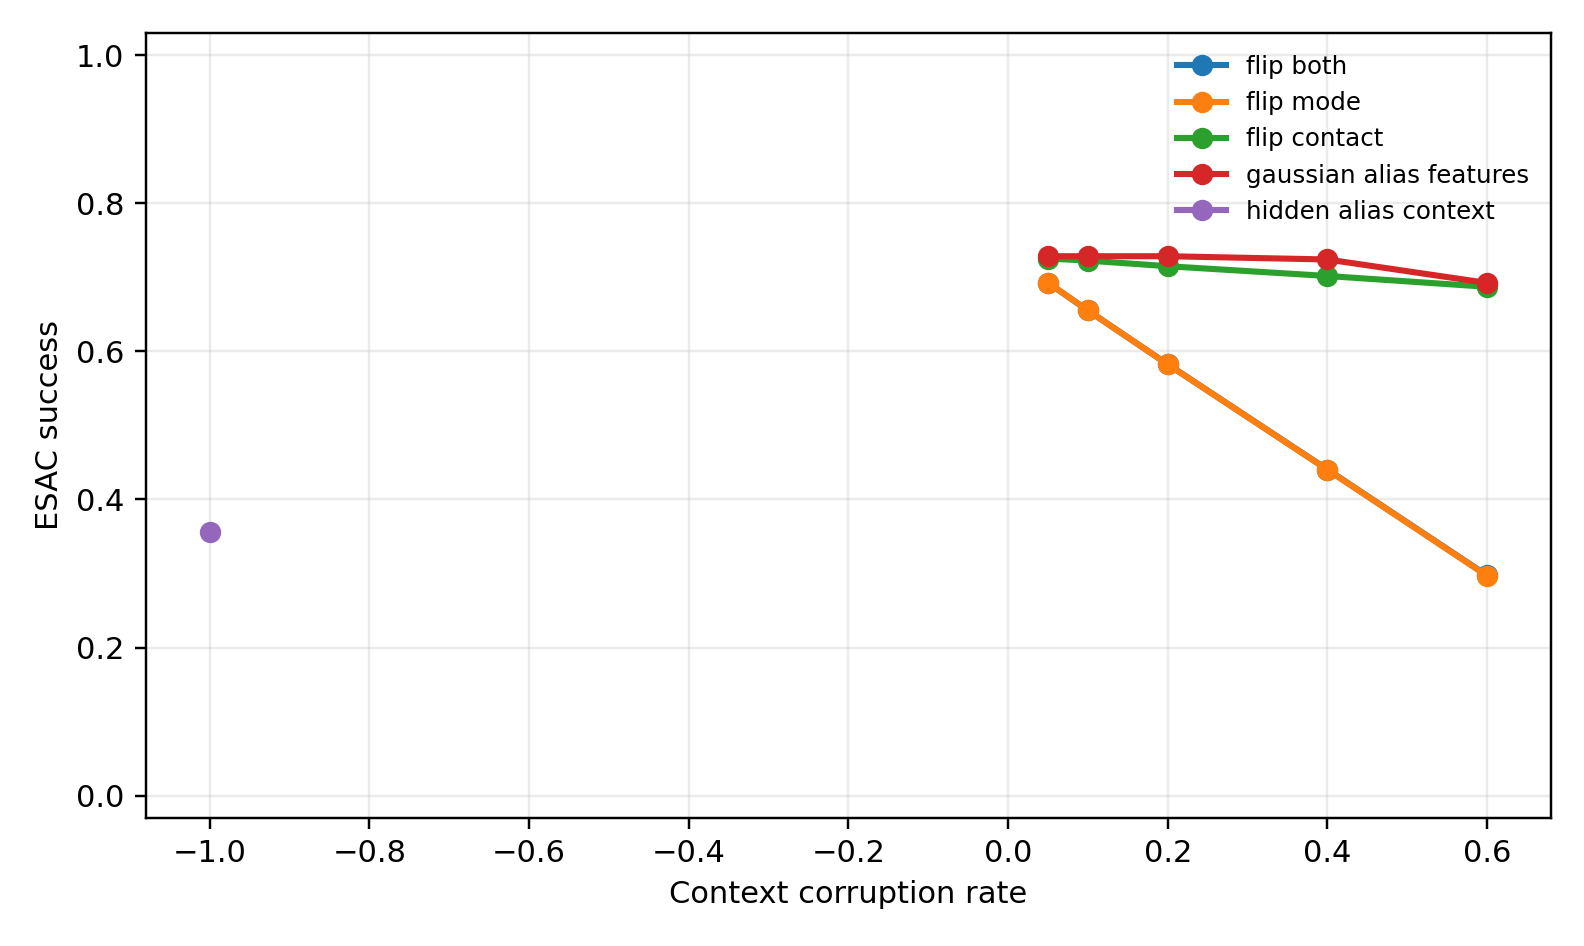
\includegraphics[width=0.78\linewidth]{figures/context_reliability.png}
    \caption{ESAC is an effect-chart repair, not an oracle. It depends mostly
    on the mode variable in this simulator: flipping mode or both alias
    variables degrades strongly, contact-only flips matter less, and hidden
    alias context collapses the chart predictor.}
    \label{fig:context}
\end{figure}

\begin{table}[t]
\centering
\caption{Context reliability at alias strength $1.25$, averaged over 10 seeds.}
\label{tab:context}
\resizebox{\linewidth}{!}{
\begin{tabular}{lccc}
\toprule
Condition & 20\% corruption & 40\% corruption & 60\% corruption \\
\midrule
Flip both mode/contact & 0.582 & 0.440 & 0.297 \\
Flip mode only & 0.582 & 0.440 & 0.297 \\
Flip contact only & 0.715 & 0.702 & 0.687 \\
Gaussian alias-feature noise & 0.728 & 0.724 & 0.692 \\
Hidden alias context & \multicolumn{3}{c}{0.356} \\
\bottomrule
\end{tabular}}
\end{table}

The context suite clarifies the assumption. In this simulator, the mode feature
is the dominant alias-resolving variable. Flipping mode or both variables at
20\% reduces ESAC from 0.728 to 0.582, and 40\% corruption reduces it to 0.440.
Hiding the alias context gives 0.356. Contact-only flips matter less because
contact contributes a smaller part of the effect split. This is not a weakness
to hide: a real ESAC audit must identify which observation variables actually
resolve the fiber.

\subsection{Token Granularity}

\begin{figure}[t]
    \centering
    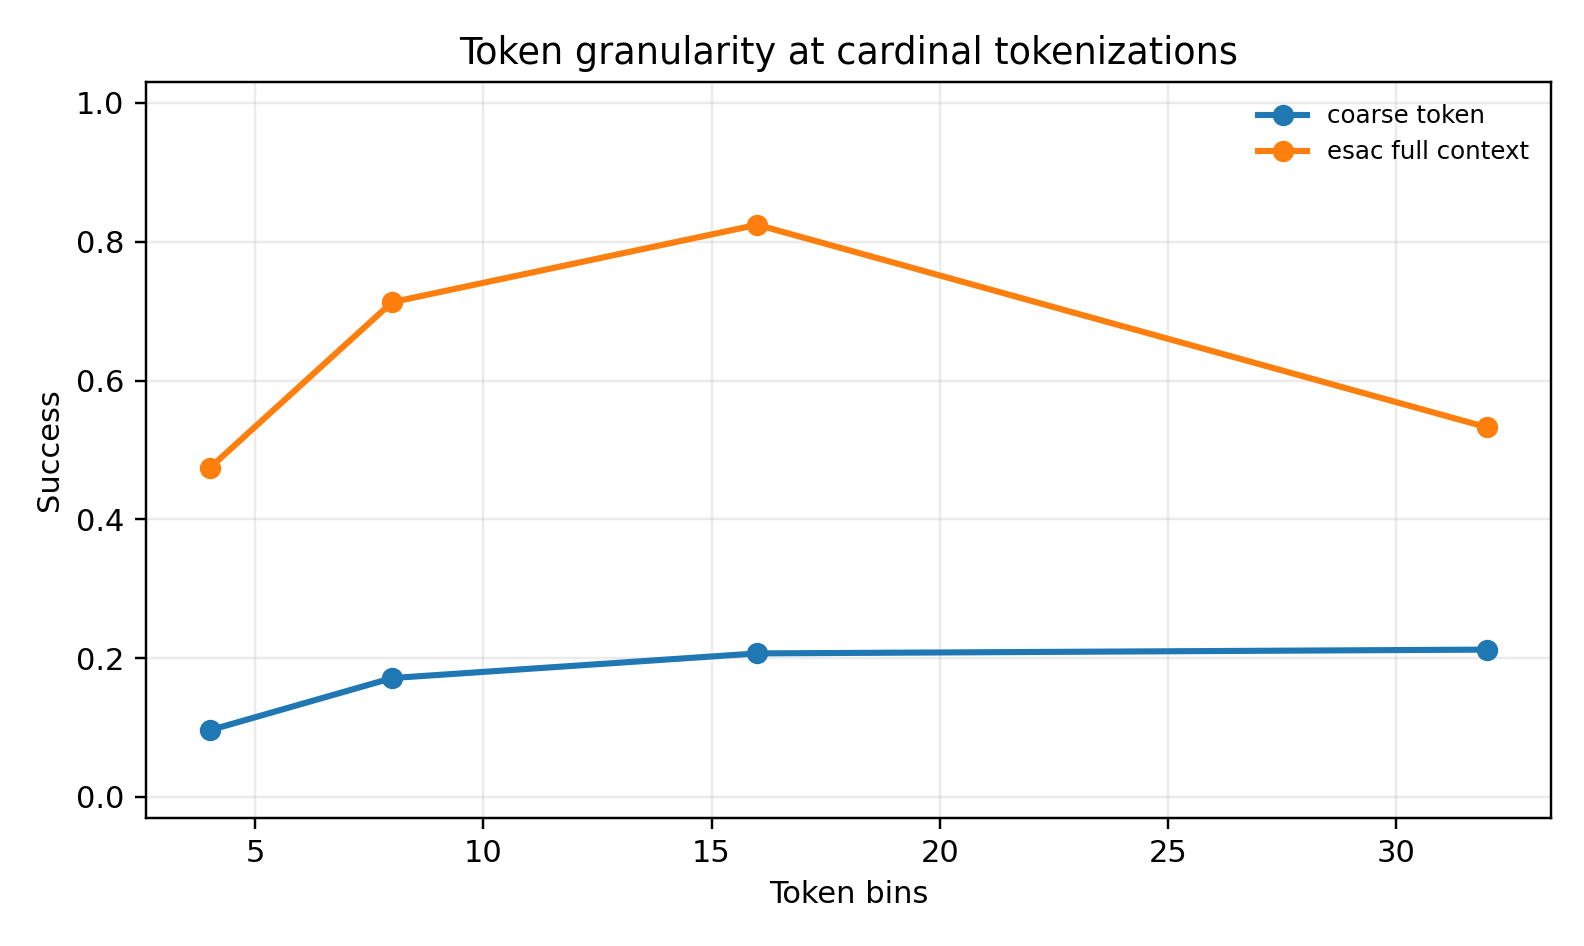
\includegraphics[width=0.78\linewidth]{figures/token_granularity.png}
    \caption{Token granularity controls. Coarser cardinal tokens increase
    aliasing. Oracle mode/contact tokenization partially removes the bottleneck.
    Very fine cardinal bins can become data-hungry for chart prediction.}
    \label{fig:token}
\end{figure}

\begin{table}[t]
\centering
\caption{Tokenization controls at alias strength $1.25$, averaged over 8 seeds.}
\label{tab:token}
\resizebox{\linewidth}{!}{
\begin{tabular}{lcc}
\toprule
Tokenization & Coarse token success & ESAC full-context success \\
\midrule
Single token & 0.000 & 0.033 \\
4 cardinal bins & 0.092 & 0.431 \\
8 cardinal bins & 0.146 & 0.712 \\
16 cardinal bins & 0.185 & 0.826 \\
32 cardinal bins & 0.191 & 0.522 \\
8 bins plus oracle mode/contact & 0.760 & 0.867 \\
\bottomrule
\end{tabular}}
\end{table}

Table~\ref{tab:token} contains two boundary controls. First, when tokenization
is made absurdly coarse by collapsing everything into one token, ESAC cannot
recover reliable chart choice and reaches only 0.033. Second, when the token
itself includes mode/contact, coarse-token success rises to 0.760. This proves
the problem is not discreteness by itself. The problem is a tokenization that
omits effect-relevant distinctions. The drop at 32 cardinal bins is also useful:
finer tokenization can leave too little data per token for reliable chart
prediction.

\subsection{Chart Count and Data Scale}

\begin{figure}[t]
    \centering
    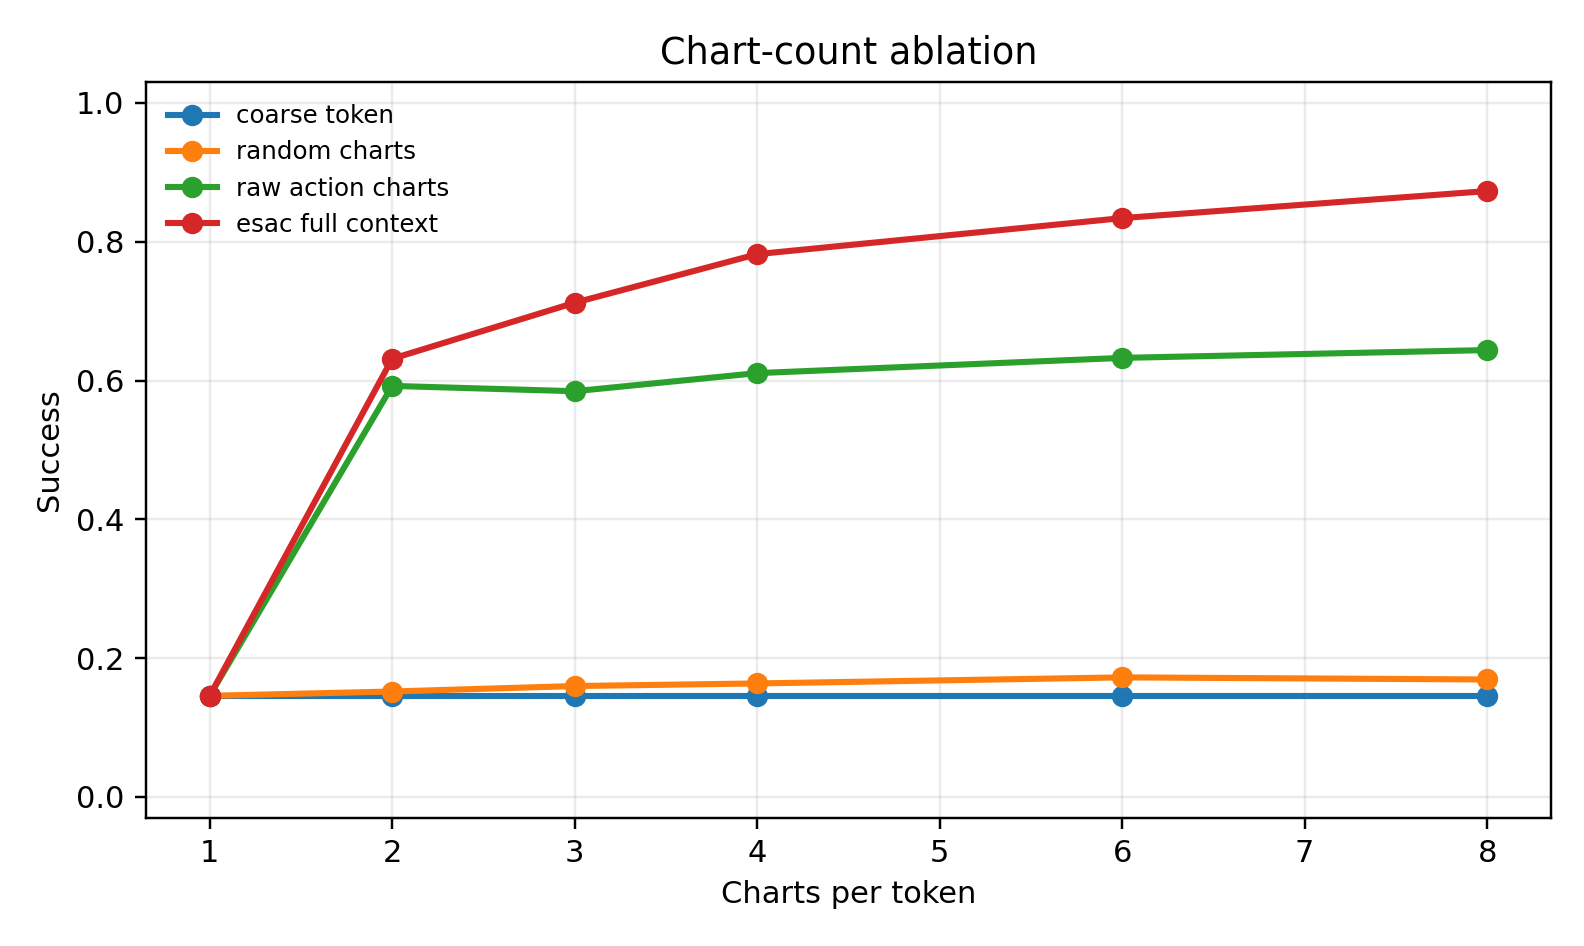
\includegraphics[width=0.49\linewidth]{figures/chart_count_ablation.png}
    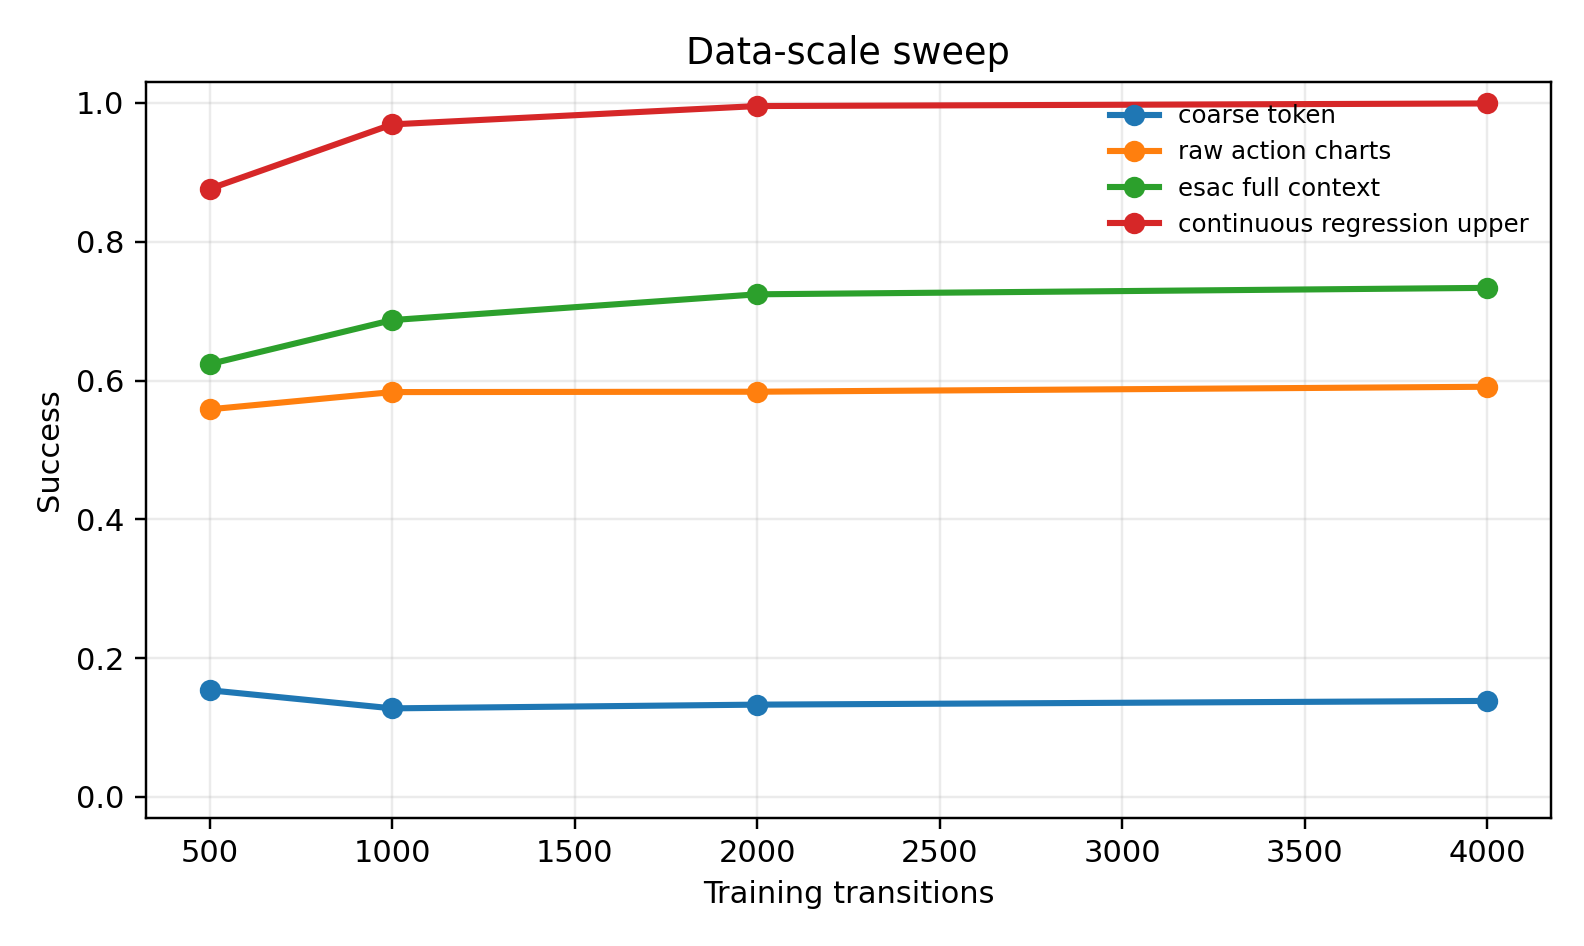
\includegraphics[width=0.49\linewidth]{figures/data_scale.png}
    \caption{Left: ESAC improves as chart count increases; random charts remain
    near coarse-token performance and raw action charts are consistently weaker.
    Right: ESAC needs transition data, while continuous regression is an upper
    baseline that bypasses token repair.}
    \label{fig:chartsdata}
\end{figure}

\begin{table}[t]
\centering
\caption{Chart-count ablation at alias strength $1.25$, averaged over 8 seeds.}
\label{tab:charts}
\resizebox{\linewidth}{!}{
\begin{tabular}{rrrr}
\toprule
Charts per token & Random charts & Raw action charts & ESAC effect charts \\
\midrule
1 & 0.146 & 0.146 & 0.146 \\
2 & 0.152 & 0.592 & 0.631 \\
3 & 0.160 & 0.585 & 0.712 \\
4 & 0.164 & 0.611 & 0.782 \\
6 & 0.172 & 0.633 & 0.834 \\
8 & 0.169 & 0.644 & 0.873 \\
\bottomrule
\end{tabular}}
\end{table}

The chart ablation demonstrates that the repair is not merely adding more
clusters. Random charts stay near coarse-token performance. Raw action charts
help but saturate below ESAC. Effect charts improve from 0.631 with two charts
to 0.873 with eight charts. This is a design tradeoff: more charts reduce
within-chart effect radius but require more data and a reliable chart
predictor.

The data-scale suite shows the same tradeoff from another angle. With 500
training transitions, ESAC reaches 0.624; with 4,000 it reaches 0.734. The
coarse token baseline stays near 0.13 because its problem is not data scarcity
but the one-prototype fiber collapse. Continuous regression rises from 0.876 to
0.999, which is why it is reported as an upper comparator rather than as a
token-repair baseline.

\subsection{Distribution Shift, Metrics, and Thresholds}

\begin{figure}[t]
    \centering
    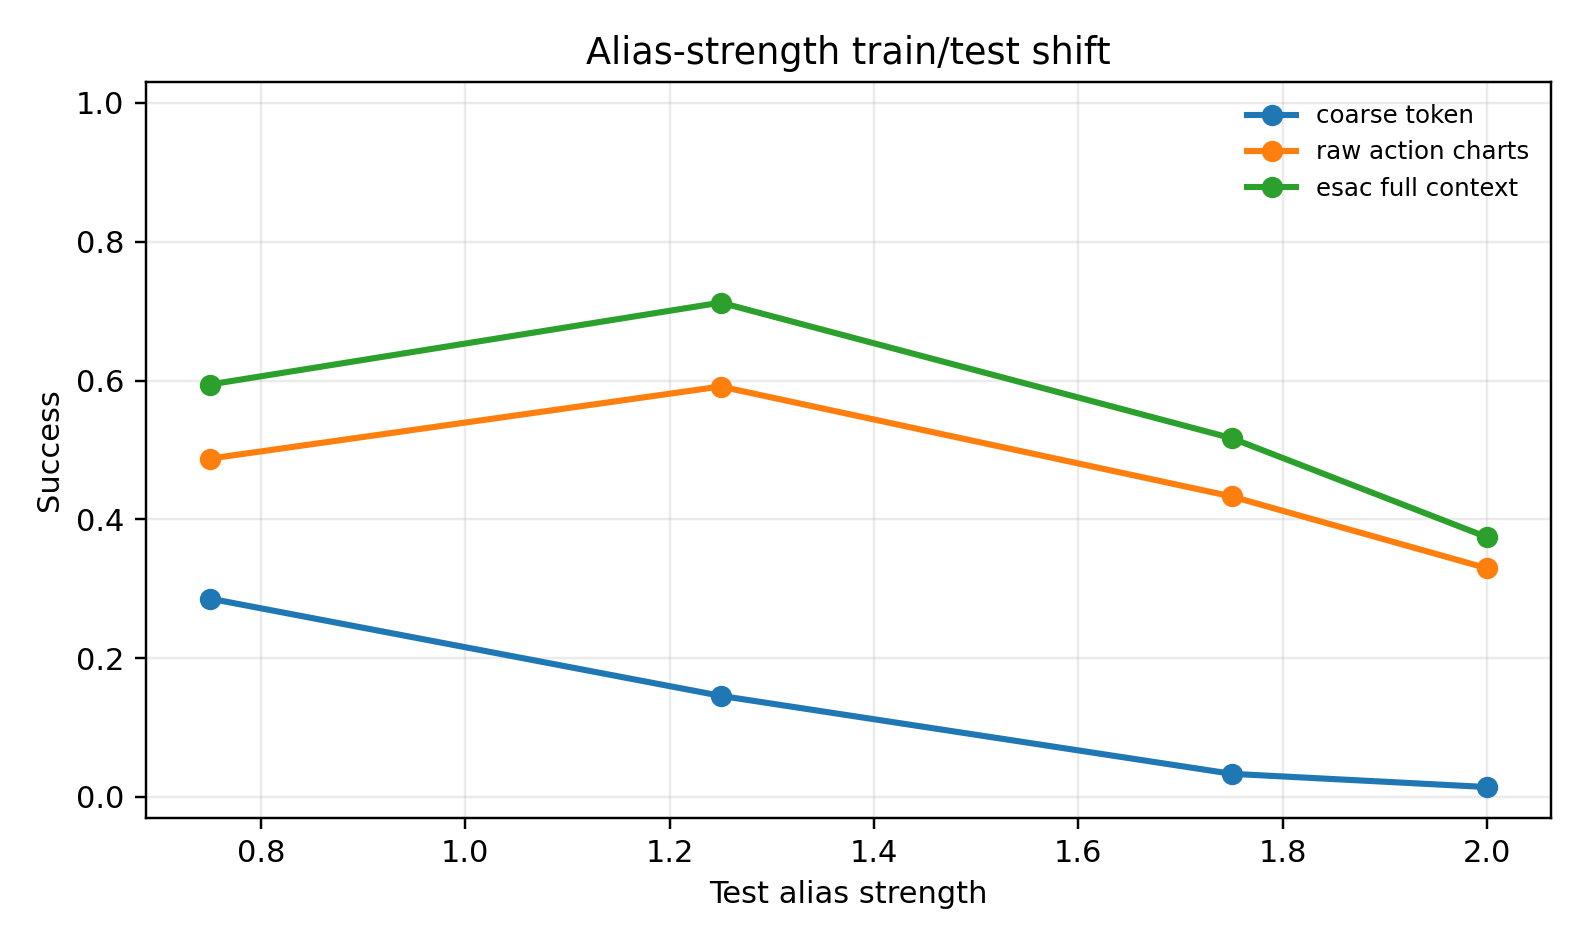
\includegraphics[width=0.49\linewidth]{figures/alias_shift.png}
    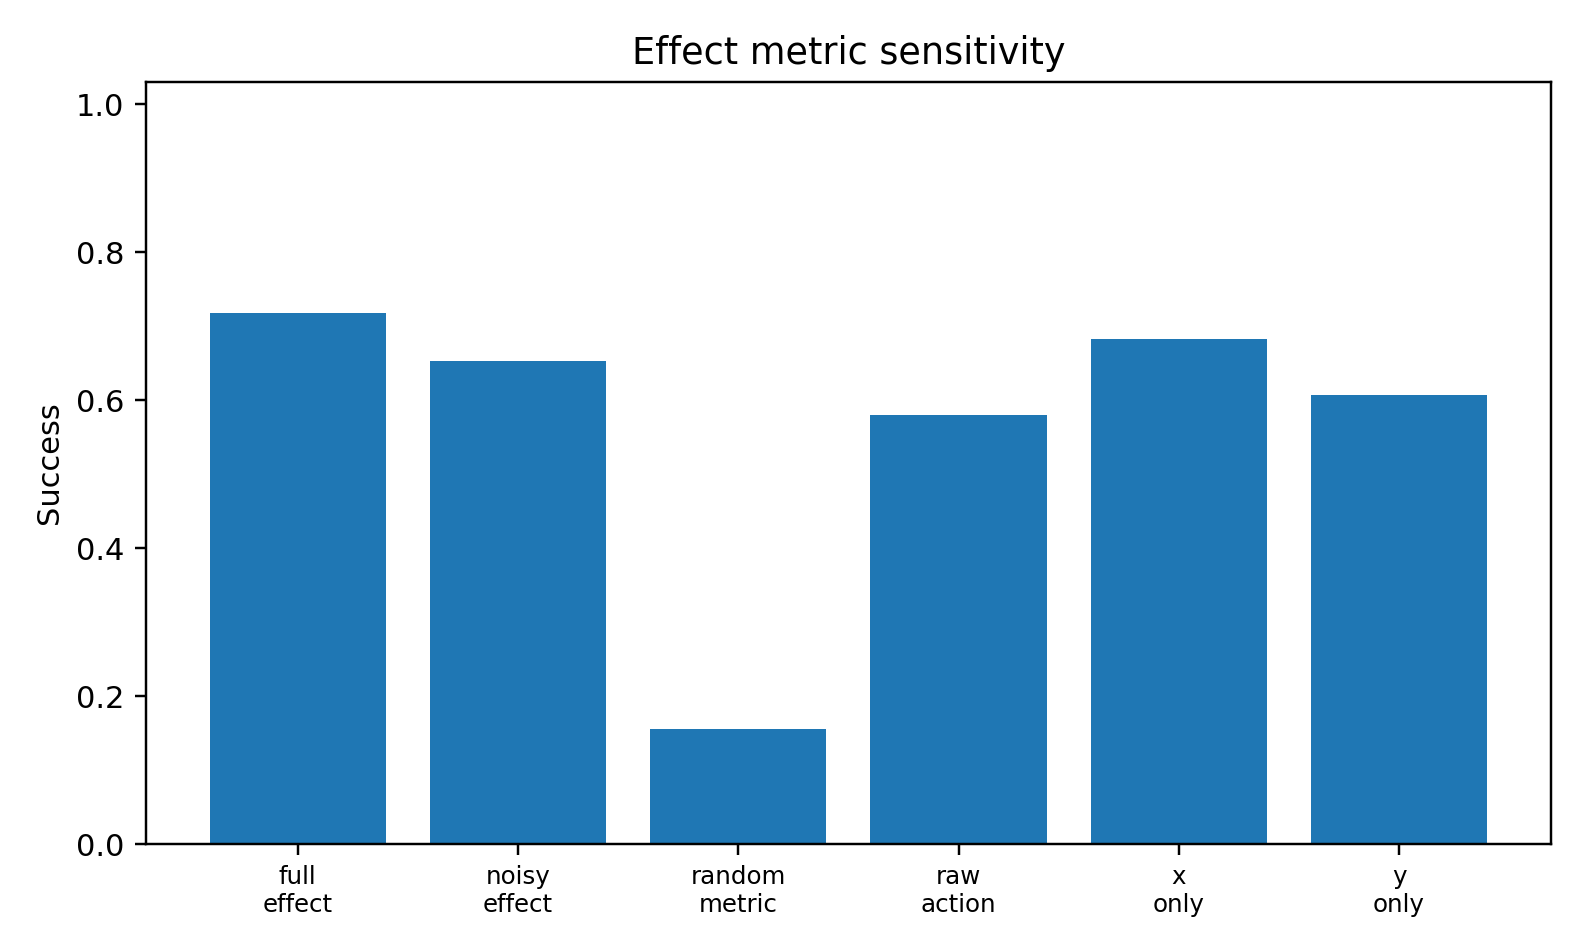
\includegraphics[width=0.49\linewidth]{figures/effect_metric_sensitivity.png}
    \caption{Left: train/test alias-strength shift. ESAC trained at alias
    strength 1.25 still helps under stronger test aliasing, but degrades. Right:
    the effect metric matters. Random or raw-action charting is weaker than
    the task-relevant full effect metric.}
    \label{fig:shiftmetric}
\end{figure}

\begin{figure}[t]
    \centering
    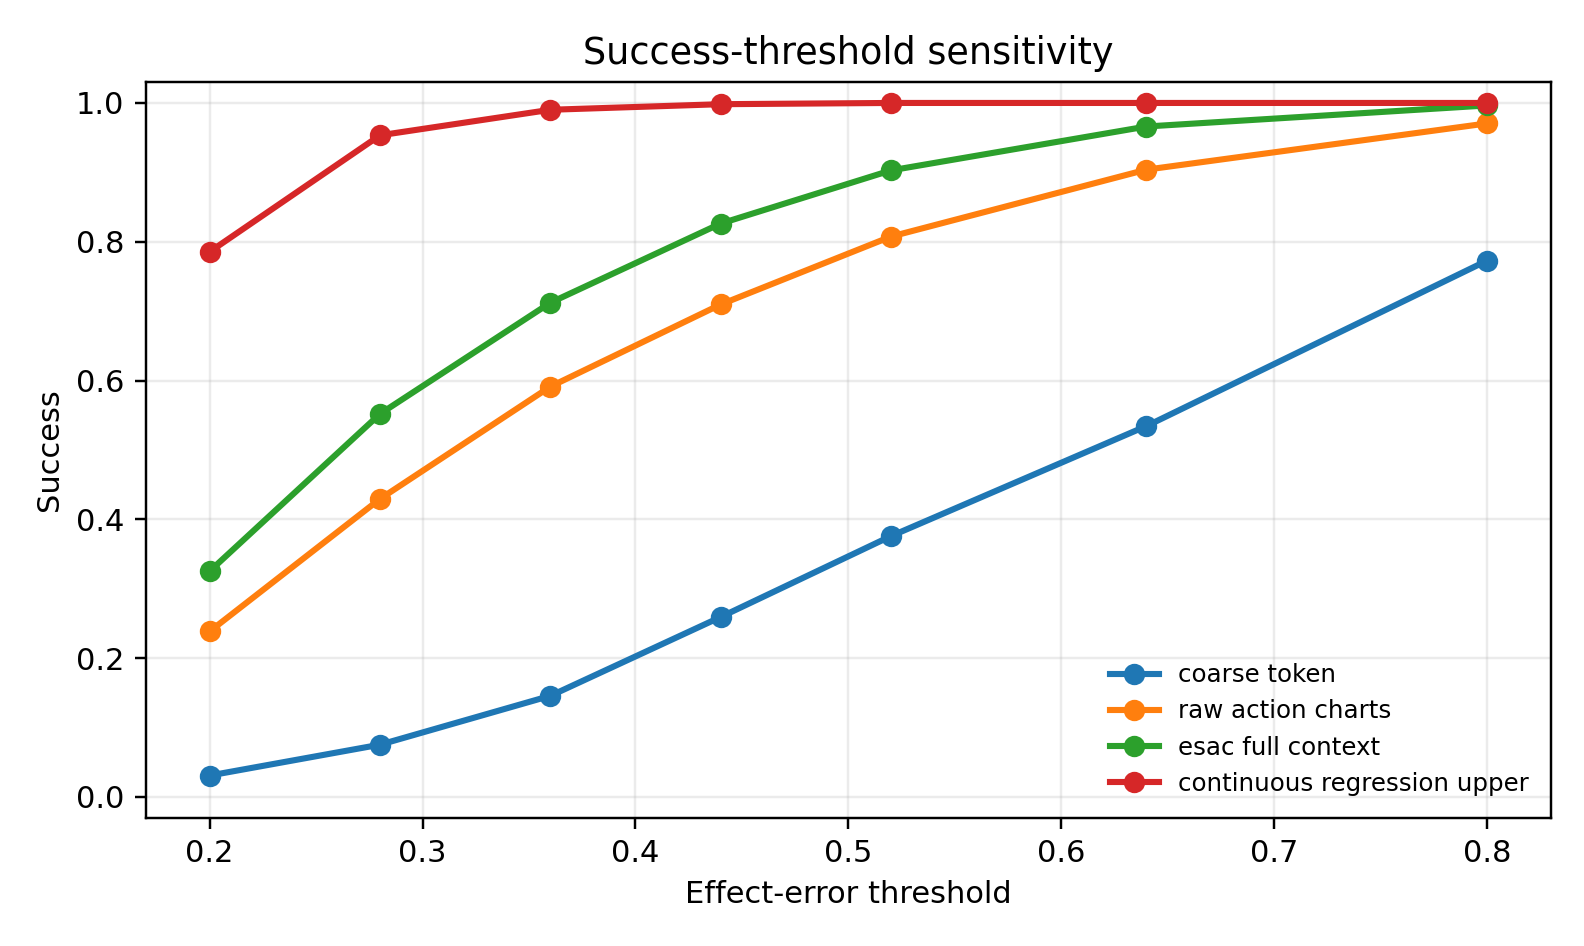
\includegraphics[width=0.78\linewidth]{figures/threshold_sensitivity.png}
    \caption{Threshold sensitivity at alias strength $1.25$. ESAC retains a
    large advantage over coarse tokens across strict and lenient success
    thresholds.}
    \label{fig:threshold}
\end{figure}

When training at alias strength 1.25 and testing at strength 2.0, ESAC reaches
0.374 while coarse tokens reach 0.014. The repair helps under shift but does
not make the model distribution-robust. Effect-metric sensitivity is similarly
important: full-effect charting reaches 0.718, noisy-effect charting 0.653,
raw-action charting 0.580, and random-metric charting 0.156. The threshold
sweep shows that the main claim does not depend on one arbitrary tolerance:
at threshold 0.20, coarse tokens reach 0.031 and ESAC reaches 0.325; at
threshold 0.64, coarse tokens reach 0.534 and ESAC reaches 0.966.

\subsection{Negative Controls}

\begin{table}[t]
\centering
\caption{Negative and boundary controls, averaged over 8 seeds.}
\label{tab:negative}
\resizebox{\linewidth}{!}{
\begin{tabular}{lccc}
\toprule
Control & Coarse token & ESAC full context & ESAC hidden context \\
\midrule
No alias strength & 0.713 & 0.978 & 0.710 \\
Oracle mode token & 0.631 & 0.834 & 0.743 \\
Oracle mode/contact token & 0.760 & 0.868 & 0.868 \\
Single-token alias & 0.000 & 0.032 & 0.017 \\
Strong alias, hidden context & 0.116 & 0.681 & 0.356 \\
\bottomrule
\end{tabular}}
\end{table}

Table~\ref{tab:negative} prevents overclaiming. ESAC is not a universal
solution to bad interfaces. A single-token collapse gives it almost nothing to
recover. Oracle tokenization that includes alias variables makes coarse tokens
much stronger. Hidden context still fails. These controls are the reason the
paper's claim is conditional rather than universal.

\section{Discussion}

\paragraph{What the experiments support.}
The experiments support a mechanism claim. When a token fiber has large
task-relevant effect diameter, one prototype per token is physically
non-identifiable. Splitting the fiber by observed effects repairs much of the
damage when the observation contains the variables needed to select a chart.
The evidence also shows that the repair target matters: raw action charts and
random charts are weaker than effect charts.

\paragraph{What the experiments do not support.}
The experiments do not prove that current deployed VLAs have severe aliasing,
nor that ESAC is state of the art on a real robot. They do not prove that the
chosen effect metric is easy to define for every task. They do not beat a
continuous policy that bypasses tokenization. They do not solve chart selection
when the alias-resolving context is absent. These limitations are not side
notes; they define the research boundary.

\paragraph{Why token accuracy can mislead.}
If a model predicts the demonstration token but the token hides several effects,
token accuracy can be high while control is underdetermined. This is analogous
to a semantic label that names a skill without specifying the force mode,
contact side, or nullspace choice that makes the skill work. Reporting effect
diameter inside action tokens would catch this failure before deployment.

\paragraph{How a real audit would look.}
A real VLA audit would log emitted token, decoded low-level action, observation
features, and measured transition effect. For each token, the audit would
estimate effect radius conditioned on task and local state. Tokens with large
radius would be flagged. A repair could add chart ids, refine the tokenizer, add
context to the action interface, or bypass the token with a continuous decoder.
ESAC is one repair; the broader demand is that action tokens be certified by
physical effects.

\section{Limitations}

The study is synthetic. The simulator isolates one mechanism but does not
capture real robot contact dynamics, sensing, latency, controller safety, or
data collection. The literature audit is broad but mostly metadata/abstract
based at scale. The effect metric is engineered and two-dimensional. Real tasks
may require force, pose, contact, and object-state effects. Chart selection
requires alias-resolving observations; when those observations are hidden or
corrupted, ESAC degrades. Continuous-action policies can avoid this exact
many-to-one bottleneck. Finally, ESAC adds an audit and decoding layer rather
than replacing the need for a strong policy.

\section{Conclusion}

Robot action tokens should not be treated as physically atomic merely because a
foundation model can predict them. The right question is whether a token's
fiber has small next-state effect diameter under local dynamics. If it does
not, the token is non-identifiable for control. ESAC is a first repair: split
action tokens by physical effect charts and decode with the observations that
resolve the fiber. The result is a synthetic mechanism paper with a practical
demand for future robot foundation models: report, audit, and repair
action-fiber aliasing.

\bibliographystyle{iclr2026_conference}
\bibliography{references}

\appendix
\renewcommand{\thesection}{A.\arabic{section}}

\section{Full-Scale Artifact Inventory}

\begin{table}[h]
\centering
\caption{Full-scale artifact inventory.}
\label{tab:inventory}
\resizebox{\linewidth}{!}{
\begin{tabular}{lrr}
\toprule
Suite file & Compact rows & Purpose \\
\midrule
\texttt{main\_sweep.csv} & 540 & Alias strength, six methods, ten seeds \\
\texttt{context\_reliability.csv} & 250 & Mode/contact corruption and hidden context \\
\texttt{token\_granularity.csv} & 576 & Token bins and oracle tokenization controls \\
\texttt{chart\_ablation.csv} & 192 & Chart count, random charts, raw charts, ESAC \\
\texttt{data\_scale.csv} & 192 & Training-transition scale \\
\texttt{alias\_shift.csv} & 384 & Train/test alias-strength mismatch \\
\texttt{effect\_metric.csv} & 48 & Effect metric misspecification \\
\texttt{threshold\_sensitivity.csv} & 224 & Success threshold sweep \\
\texttt{negative\_controls.csv} & 120 & Boundary and negative controls \\
\bottomrule
\end{tabular}}
\end{table}

The total compact row count is 2,526. The total evaluated prediction count,
counting each row's test set, is 2,005,200. The artifact stores compact metrics
and figures, not raw train/test arrays.

\section{Reproducibility Commands}

The full-scale runner is:

\begin{verbatim}
python scripts/run_full_scale_experiments.py --suite main
  --seed-scale 10 --train-rows 2600 --test-rows 1000 --fresh
python scripts/run_full_scale_experiments.py --suite context
  --seed-scale 10 --train-rows 2600 --test-rows 1000
python scripts/run_full_scale_experiments.py --suite token
  --seed-scale 8 --train-rows 1600 --test-rows 700
python scripts/run_full_scale_experiments.py --suite charts
  --seed-scale 8 --train-rows 1600 --test-rows 700
python scripts/run_full_scale_experiments.py --suite data
  --seed-scale 8 --train-rows 1600 --test-rows 700
python scripts/run_full_scale_experiments.py --suite shift
  --seed-scale 8 --train-rows 1600 --test-rows 700
python scripts/run_full_scale_experiments.py --suite metric
  --seed-scale 8 --train-rows 1600 --test-rows 700
python scripts/run_full_scale_experiments.py --suite threshold
  --seed-scale 8 --train-rows 1600 --test-rows 700
python scripts/run_full_scale_experiments.py --suite negative
  --seed-scale 8 --train-rows 1600 --test-rows 700
python scripts/run_full_scale_experiments.py --suite summarize
  --seed-scale 8 --train-rows 1600 --test-rows 700
\end{verbatim}

The manuscript is rebuilt from \texttt{paper/} with:

\begin{verbatim}
pdflatex -interaction=nonstopmode -halt-on-error main.tex
bibtex main
pdflatex -interaction=nonstopmode -halt-on-error main.tex
pdflatex -interaction=nonstopmode -halt-on-error main.tex
\end{verbatim}

\section{Additional Formal Notes}

\paragraph{State-conditioned tokens.}
The setup allows $q_s$ rather than only $q$. This matters because a tokenization
that includes embodiment, controller mode, or contact context can shrink fiber
diameter. The oracle mode/contact tokenization control is exactly this case. It
raises coarse-token success because the token no longer hides the dominant
alias variable.

\paragraph{Effect-radius estimation.}
The empirical radius $\widehat R(z)$ is a lower-resolution proxy for diameter.
It is less sensitive to outliers than the maximum pairwise distance and easier
to estimate from logs. A deployment audit could use both: radius for routine
monitoring and high-quantile pairwise distance for safety-critical tokens.

\paragraph{Expected loss.}
If task loss is Lipschitz in effect error, then reducing within-chart effect
diameter directly tightens a bound on one-step task loss. This is why ESAC
clusters by effects rather than raw action coordinates.

\section{Implementation Details}

The simulator constructs a local dynamics matrix $B(s)\in\mathbb{R}^{2\times4}$
from angle, mode, contact, friction, and embodiment. The expert action is the
minimum-norm action producing the desired effect, plus nullspace jitter and
small noise. The nullspace jitter is intentional. It creates cases where action
vectors differ without changing the object effect, so raw-action clustering can
split the wrong thing.

The ESAC chart predictor is a decision tree in the full-scale runner. This is a
deliberately simple choice. The paper's claim is not that this predictor is
optimal; the claim is that the chart target should be effect-based. A stronger
implementation could use calibrated classifiers, nearest-neighbor retrieval,
mixture density heads, or local continuous decoders.

\section{Additional Suite Interpretations}

\paragraph{Alias shift.}
Training at alias strength 1.25 and testing at 2.0 reduces ESAC to 0.374. The
same shift nearly destroys coarse tokens, which reach 0.014. ESAC is therefore
more robust than a single prototype but not distribution invariant.

\paragraph{Effect metric sensitivity.}
Full-effect charting reaches 0.718 in the metric suite. Raw-action charting
reaches 0.580, noisy-effect charting 0.653, and random-metric charting 0.156.
This confirms that effect separation needs the right physical measurement.

\paragraph{Threshold sensitivity.}
At a strict threshold of 0.20, ESAC reaches 0.325 and coarse tokens 0.031. At a
lenient threshold of 0.80, ESAC reaches 0.996 and coarse tokens 0.773. The
advantage persists across thresholds, although the absolute success rates
change.

\section{Failure Narratives}

\paragraph{No alias-resolving observation.}
If the observation does not contain the variable that selects the chart, ESAC
can cluster the training fiber but cannot choose the correct chart at test time.
This is the hidden-context ablation.

\paragraph{Bad effect metric.}
If $\phi$ ignores the effect dimension that controls success, the audit can
miss aliasing or split irrelevant variation. Random-metric charting is the
extreme negative control.

\paragraph{Over-fine tokenization.}
Finer tokens can reduce aliasing but create data fragmentation. The 32-bin
control has higher coarse-token success than 8 bins but weaker ESAC than 16
bins because chart prediction becomes data-hungry.

\paragraph{Continuous bypass.}
If a policy emits a continuous action with enough context, it can bypass the
many-to-one token lower bound. This does not refute the audit; it identifies a
different interface.

\section{Practical Audit Checklist}

A practitioner auditing an action-token robot dataset should:

\begin{enumerate}[leftmargin=1.4em]
    \item Choose task-relevant effect features.
    \item Group logged transitions by emitted action token.
    \item Estimate within-token effect radius and high-quantile effect
    distance.
    \item Inspect tokens with high effect radius.
    \item Check whether observations contain the variables that separate the
    effect clusters.
    \item Compare raw-action clusters with effect clusters.
    \item Add chart ids, refine tokenization, or bypass tokens for aliased
    fibers.
    \item Re-audit residual chart effect radius after repair.
\end{enumerate}

\section{Claim Audit Checklist}

The claim is credible only if these statements remain visible:

\begin{itemize}[leftmargin=1.4em]
    \item The paper is about tokenized or language-like action interfaces, not
    all robot policies.
    \item Continuous-action policies are an upper comparator, not a baseline
    ESAC must beat.
    \item ESAC requires measured transition effects during audit/training.
    \item ESAC requires alias-resolving observations at test time.
    \item Oracle tokenization can remove much of the failure.
    \item Single-token collapse can be too severe for ESAC to repair.
    \item The effect metric is task-dependent and can be wrong.
    \item The evidence is synthetic and mechanism-level.
\end{itemize}

\section{Detailed Suite Descriptions}

This appendix records the purpose of each suite. The suites are not nine
unrelated benchmarks; they are nine ways of interrogating the same mechanism.
The main sweep asks whether aliasing hurts coarse tokens. The boundary controls
ask whether the hurt disappears when the token interface is repaired. The
negative controls ask whether ESAC fails when its assumptions are violated.

\paragraph{Main alias-strength sweep.}
The main suite varies alias strength from 0.0 to 2.0. Alias strength controls
how strongly the hidden wrist/force channels affect object motion through the
local dynamics matrix. At strength 0.0, the coarse token still loses some
information but the collapse is mild. At strength 1.25, the token fiber contains
physically separated effects. At strength 2.0, the same cardinal token can
represent strongly different object displacements. The sweep is the primary
test of the lower-bound story: if effect diameter grows, one prototype per
token should fail.

\paragraph{Context reliability.}
The context suite asks whether the chart predictor sees the variable that
selects a chart. In the simulator, mode and contact are the alias-resolving
features, with mode more influential than contact. The suite flips mode,
contact, both, or adds Gaussian feature noise. It also includes the hidden
context ablation. This suite prevents an overclaim that ESAC repairs token
fibers without the observations needed to choose the right local chart.

\paragraph{Token granularity.}
The token-granularity suite changes the token interface itself. Four cardinal
bins make tokens very coarse. Eight bins are the default. Sixteen and thirty-two
bins make the angular tokenization finer. Oracle tokenization appends mode and
contact to the token id, making the token interface more physically specific.
The single-token control collapses every action into one token. This suite asks
whether the problem comes from tokenization as such or from omitting the
effect-relevant variables.

\paragraph{Chart-count ablation.}
The chart-count suite varies the number of charts allowed inside each token. A
single chart is equivalent to a token prototype. More charts can reduce
within-chart effect radius but also demand more training data and a more
accurate chart predictor. The random-chart baseline uses the same chart budget
but assigns meaningless chart labels; it checks whether simply adding clusters
is enough.

\paragraph{Data-scale sweep.}
ESAC needs transition logs to estimate effects and train a chart predictor. The
data-scale suite sweeps training transitions while keeping the test count fixed.
The result distinguishes representation failure from data scarcity. Coarse
tokens remain weak because a single prototype cannot represent the fiber.
ESAC improves with more transitions because it can learn effect charts and
chart selection more reliably.

\paragraph{Alias-strength shift.}
The shift suite trains at one alias strength and tests at another. This is a
distribution-shift stress, not a main claim. It asks whether ESAC trained under
one degree of physical separation still helps when the separation grows or
shrinks. The answer is mixed: ESAC still helps, but it degrades under stronger
test aliasing.

\paragraph{Effect metric sensitivity.}
The metric suite changes the charting basis. Full-effect charting is the
intended ESAC target. Partial metrics keep only the $x$ or $y$ component. A
noisy metric corrupts the effect. Raw-action charting uses motor vectors rather
than effects. A random metric is the negative control. This suite tests the
claim that the physical effect metric is the semantics of the action chart.

\paragraph{Threshold sensitivity.}
The main success threshold is 0.36 effect error. The threshold suite sweeps from
strict to lenient tolerances. A robust mechanism should not depend on one
chosen threshold. The absolute success values change, but ESAC remains above
coarse tokens across the sweep.

\paragraph{Negative controls.}
The negative-control suite combines cases where the claim should shrink. With
no alias strength, coarse tokens are much less damaged. With oracle mode/contact
tokenization, the token itself carries the missing physical distinction. With a
single-token collapse, the interface is too coarse for ESAC to recover. With
strong aliasing and hidden context, the chart predictor cannot know which chart
to select.

\section{Additional Numerical Tables}

\begin{table}[h]
\centering
\caption{Main sweep success values, averaged over 10 seeds.}
\label{tab:mainsweepappendix}
\resizebox{\linewidth}{!}{
\begin{tabular}{rrrrr}
\toprule
Alias strength & Coarse token & Raw action charts & ESAC hidden context & ESAC full context \\
\midrule
0.00 & 0.713 & 0.803 & 0.728 & 0.981 \\
0.25 & 0.582 & 0.738 & 0.635 & 0.890 \\
0.50 & 0.341 & 0.712 & 0.404 & 0.789 \\
0.75 & 0.255 & 0.672 & 0.382 & 0.766 \\
1.00 & 0.184 & 0.644 & 0.364 & 0.752 \\
1.25 & 0.140 & 0.605 & 0.356 & 0.728 \\
1.50 & 0.117 & 0.564 & 0.352 & 0.710 \\
1.75 & 0.108 & 0.511 & 0.349 & 0.695 \\
2.00 & 0.102 & 0.463 & 0.345 & 0.683 \\
\bottomrule
\end{tabular}}
\end{table}

\begin{table}[h]
\centering
\caption{Data-scale readout at alias strength $1.25$, averaged over 8 seeds.}
\label{tab:datascaleappendix}
\resizebox{\linewidth}{!}{
\begin{tabular}{rrrr}
\toprule
Training transitions & Coarse token & ESAC full context & Continuous upper \\
\midrule
500 & 0.154 & 0.624 & 0.876 \\
1,000 & 0.128 & 0.687 & 0.969 \\
2,000 & 0.133 & 0.724 & 0.996 \\
4,000 & 0.138 & 0.734 & 0.999 \\
\bottomrule
\end{tabular}}
\end{table}

\begin{table}[h]
\centering
\caption{Effect metric sensitivity at alias strength $1.25$, averaged over 8 seeds.}
\label{tab:metricappendix}
\resizebox{\linewidth}{!}{
\begin{tabular}{lr}
\toprule
Charting metric & Success \\
\midrule
Full task-relevant effect & 0.718 \\
$x$-only effect & 0.683 \\
$y$-only effect & 0.607 \\
Noisy effect & 0.653 \\
Raw action vector & 0.580 \\
Random metric & 0.156 \\
\bottomrule
\end{tabular}}
\end{table}

\begin{table}[h]
\centering
\caption{Threshold sensitivity at alias strength $1.25$, averaged over 8 seeds.}
\label{tab:thresholdappendix}
\resizebox{\linewidth}{!}{
\begin{tabular}{rrr}
\toprule
Effect-error threshold & Coarse token & ESAC full context \\
\midrule
0.20 & 0.031 & 0.325 \\
0.28 & 0.075 & 0.552 \\
0.36 & 0.146 & 0.712 \\
0.44 & 0.259 & 0.826 \\
0.52 & 0.376 & 0.903 \\
0.64 & 0.534 & 0.966 \\
0.80 & 0.773 & 0.996 \\
\bottomrule
\end{tabular}}
\end{table}

\section{Simulator Equations}

This section gives more detail about the synthetic environment. The simulator
is not meant to be a complete physical model. It is a controlled construction
where a specific abstraction failure can be toggled.

The command angle $\theta$ defines a nominal direction
\[
    d(\theta)=(\cos\theta,\sin\theta)
\]
and an orthogonal direction
\[
    n(\theta)=(-\sin\theta,\cos\theta).
\]
The desired target effect is the nominal direction plus an alias-sensitive
orthogonal component and a smaller contact component,
\[
    e^\star
    =
    d(\theta)
    +
    \alpha(0.72+0.36\rho)m\,n(\theta)
    +
    0.22 c(1-0.25|\gamma|)
    (\cos 2\theta,\sin 2\theta),
\]
where $\alpha$ is alias strength, $\rho$ is friction, $m\in\{-1,1\}$ is mode,
$c\in\{-1,1\}$ is contact sign, and $\gamma$ is clearance. The token keeps only
a coarse bin of $\theta$ by default. It therefore omits $m$ and $c$, even though
they change the target effect.

The local dynamics are linear,
\[
    e=B(s)a,
\]
with $a\in\mathbb{R}^4$. The first two action channels are planar command
channels. The last two are hidden wrist/force channels. Their gains depend on
mode, contact, friction, and embodiment. The expert action is the
minimum-norm solution $a^\star=B(s)^\dagger e^\star$ plus nullspace jitter and
small motor noise. The nullspace jitter is essential: it creates action-vector
differences that are not effect differences, so raw action clustering can be
misled.

The success metric is
\[
    \|B(s)\hat a-e^\star\|_2 < \tau,
\]
with $\tau=0.36$ in the main tables. Threshold sensitivity is reported because
no single tolerance should carry the entire claim.

\section{Real Dataset Audit Protocol}

The synthetic environment is only a mechanism test. A real audit of a VLA or
robot foundation model would need to operate on logged robot data. The minimum
log fields are:

\begin{itemize}[leftmargin=1.4em]
    \item observation or compact state features before the action,
    \item emitted token or skill id,
    \item decoded low-level action or controller command,
    \item executed low-level action after safety/controller modification,
    \item next observation or measured transition effect,
    \item task id and local success tolerance,
    \item embodiment/controller metadata.
\end{itemize}

The audit would group transitions by token and task context, compute effect
features, and estimate within-token effect radius. High-radius fibers would be
inspected manually and automatically. The key diagnostic plots would show
effect clusters inside one token, raw-action clusters inside one token, and the
observation variables that predict the effect clusters. If the effect clusters
are separable by available observations, a chart repair is plausible. If the
clusters are not separable, the action interface needs a richer token, more
state, or a continuous action head.

The audit should also compare against a refined tokenization. If adding
controller mode, contact side, gripper state, or embodiment id to the token
collapses the effect radius, then the original token was underspecified. If
effect radius remains high after adding those variables, then the problem is
not merely missing metadata and may require a new action representation.

\section{Design Alternatives}

\paragraph{Refine the tokenizer.}
The simplest repair is to define a better token. The oracle mode/contact
control shows that this can work. Refined tokenization is attractive because it
does not require a separate chart predictor. It is limited by vocabulary size
and by the designer's knowledge of which variables matter.

\paragraph{Add a chart id.}
ESAC can be viewed as adding a local chart id under a token. The token keeps its
semantic/action role, while the chart carries the physical branch. This is
useful when a token vocabulary is already baked into a model or API.

\paragraph{Use a continuous decoder.}
A continuous action head can avoid the token bottleneck. The continuous upper
baseline demonstrates this. The tradeoff is that continuous policies still need
coverage, calibration, and safety checks. They may also inherit aliasing if the
observation or latent representation has already discarded the necessary
context.

\paragraph{Use retrieval.}
Instead of clustering charts, a system could retrieve transitions from the same
token fiber whose observations match the current one. Retrieval is attractive
for rare tokens and multimodal effects. It still needs an effect audit to know
whether retrieval is necessary.

\paragraph{Use mixture density or diffusion heads.}
A richer decoder can model multimodal actions inside one token. This may
outperform prototype charts. The audit remains useful because it identifies
which tokens need multimodal decoding and which effect dimensions must be
preserved.

\section{What Would Falsify or Narrow the Claim}

The claim would be weakened by evidence that action-token fibers in real VLA
systems almost always have small effect diameter after conditioning on ordinary
observations. It would also be weakened by evidence that token-level confidence
or language grounding metrics reliably predict effect diameter. The claim would
be narrowed if effect-diameter audits were possible but chart selection failed
on real observations because alias-resolving variables are too noisy.

A stronger alternative result would show that a learned continuous or diffusion
decoder, trained on the same logs, preserves all effect distinctions without
needing explicit token-fiber audits. Even then, the audit could remain useful as
a diagnostic, but ESAC would no longer be the preferred repair. Another
falsifying direction would be a real robot benchmark where raw action charts
consistently match effect charts, implying that raw motor distance is already a
good proxy for physical effect in that setting.

\section{Reviewer-Facing Boundary Cases}

\paragraph{Is this just clustering?}
No. The chart-count ablation includes random charts, raw action charts, and
effect charts. Random charts remain near coarse-token performance. Raw action
charts help but are weaker than effect charts. The novelty is the effect
criterion for identifying and repairing aliased fibers.

\paragraph{Is this just multimodal action prediction?}
The problem is related but not identical. Multimodal prediction asks a decoder
to model several plausible actions. Action aliasing asks whether a token
interface has collapsed effects that the downstream controller must distinguish.
ESAC is an audit of the interface, not only a decoder architecture.

\paragraph{Is this unfair to tokenized policies?}
The paper includes oracle tokenization and continuous upper controls. If the
token includes the alias-resolving variables, coarse-token performance rises.
If the policy bypasses tokens with a continuous action head, it can avoid the
specific lower bound. The paper's target is not all tokenization, but
underspecified tokenization.

\paragraph{Why not always use continuous actions?}
Continuous actions are powerful, but tokens remain common in language-like
interfaces, action chunks, skill APIs, data compression, and cross-embodiment
abstractions. A system may still need to certify whether those tokens are
physically coherent, even if a continuous decoder exists downstream.

\section{Deployment Risk and Safety}

Action aliasing is safety-relevant because the robot may execute a physically
wrong member of a semantically correct action token. In contact-rich settings,
that can mean pushing on the wrong side of an object, applying the wrong force
mode, or choosing an insertion motion that jams. ESAC does not by itself make a
robot safe. It is an audit that can reveal tokens whose physical effects are
not coherent.

A deployment version should add conservative rejection. If a token has high
effect diameter and the chart predictor is uncertain, the robot should either
ask for more observation, switch to a continuous guarded controller, or decline
execution. The repair should not silently choose a chart when the observation
does not identify one. This is the practical interpretation of the hidden
context and context-corruption ablations.

\section{Extended Limitations}

Several limitations deserve emphasis. First, the simulator is two-dimensional
and one-step. Multi-step policies introduce compounding errors and may make a
currently irrelevant action component relevant later. Second, the chart
predictor is a simple decision tree. A stronger predictor may improve results,
but it may also overfit spurious context. Third, the effect metric is supplied
by the experimenter. Real tasks need validated effect features. Fourth, the
experiments do not include perception images. The context variables are already
features. Fifth, the method assumes transition logs include executed actions
and effects; many VLA datasets may not expose low-level executed controls.

These limitations are why the paper is framed as a mechanism study. The
mechanism is still valuable: a token's physical meaning is not certified by its
symbolic identity. It must be checked against the effects produced by commands
inside the token fiber.

\section{Action-Interface Taxonomy}

Action aliasing can appear in several interfaces, not only in a literal
discrete vocabulary. The formalism uses tokens because tokens are easy to name,
but the relevant property is many-to-one abstraction.

\paragraph{Language-like action words.}
A policy may emit a command such as ``push left,'' ``insert,'' or ``close
gripper.'' These words are useful at the task level but underspecified at the
contact level. A push token may hide which side of the object is loaded, which
force mode is used, or how compliance is handled. If those hidden choices
produce different object effects, the word is an aliased action token.

\paragraph{Learned discrete action codes.}
Some policies learn a discrete action vocabulary for compression or sequence
modeling. These codes may be optimized for prediction likelihood rather than
effect coherence. A code can therefore group actions that are statistically
similar in the dataset but physically different under local dynamics. ESAC
would audit such codes by transition effects rather than by reconstruction
loss.

\paragraph{Action chunks.}
Action chunking emits short sequences rather than single actions. A chunk id is
safe only if all trajectories inside the chunk fiber have similar effects under
the local state. Otherwise the chunk can hide contact timing, approach side, or
force mode. The same effect-diameter audit can be applied to chunk-level
effects or to a sequence of intermediate effects.

\paragraph{Skill APIs.}
Robots often expose a skill API: grasp, place, push, pull, slide, insert. Skill
names are tokens. Their parameters may or may not disambiguate physical
execution. If a skill call omits the contact branch that controls success, the
skill token has high effect diameter. A chart repair could add a branch id or
force the planner to pass the missing context explicitly.

\paragraph{Cross-embodiment abstractions.}
Large robot datasets often mix embodiments. A shared action token may mean
different low-level controls for different robots. If embodiment metadata is
available and used, the fiber can be split safely. If embodiment is hidden or
compressed away, the token can alias effects across robots. The oracle
tokenization control in the experiments is a small synthetic version of this
issue.

\section{Hardware Validation Design}

A useful hardware validation should preserve the causal contrast from the
synthetic study instead of attempting to validate every part of robot foundation
modeling at once. One possible design uses a planar pushing or insertion
fixture with several hidden contact modes.

\paragraph{Fixture.}
Construct objects with identical visible geometry but different hidden contact
rails or friction inserts. The robot sees the same visual prompt and receives
the same high-level action token, but the low-level wrist/force branch needed
for success differs across hidden modes. The hidden branch should produce a
measurable object displacement or insertion success effect.

\paragraph{Tokens.}
Define a coarse token such as push-left or insert-forward. The token should be
valid semantically across all fixture modes but physically underspecified.
Define oracle tokens that append the hidden mode, and continuous-action
baselines that bypass the token. These controls mirror the synthetic boundary
conditions.

\paragraph{Measurements.}
Log the emitted token, the decoded low-level action, force/torque traces,
tactile or proprioceptive context, object displacement, contact events, and
success. The effect metric can combine object displacement, final pose error,
and contact-event mismatch. The audit computes effect radius inside each token
before and after chart splitting.

\paragraph{Expected outcome.}
The expected result is ordinal rather than numeric. Coarse tokens should fail
when hidden contact mode changes the effect. Oracle tokens should improve by
carrying the missing variable. ESAC should improve only when the observation
contains enough tactile/proprioceptive information to identify the chart. If
ESAC improves even when the chart variable is hidden, the experiment is leaking
context. If ESAC does not improve when the context is visible, the effect metric
or chart predictor is inadequate.

\paragraph{Safety.}
The hardware test should use low-force guarded motions and abort thresholds.
Aliased tokens are exactly the cases where a semantically correct command can
cause a physically wrong contact. The audit should therefore be run offline
first, and online chart selection should be allowed to reject execution when
uncertain.

\section{Logging Schema for Real Audits}

\begin{table}[h]
\centering
\caption{Suggested logging schema for an action-fiber audit.}
\label{tab:logschema}
\resizebox{\linewidth}{!}{
\begin{tabular}{p{0.22\linewidth}p{0.34\linewidth}p{0.34\linewidth}}
\toprule
Field & Example & Why it matters \\
\midrule
Token or skill id & discrete action code, chunk id, skill name & Defines the fiber to audit \\
Low-level action & joint targets, Cartesian twist, force mode & Reveals variation hidden by the token \\
Executed command & post-safety command sent to controller & Separates policy output from controller modification \\
Observation context & image features, tactile state, mode, embodiment & Tests whether chart id is predictable \\
Pre/post state & object pose, contact state, force trace & Provides transition effect \\
Task tolerance & displacement or contact threshold & Defines success and alias severity \\
Metadata & robot id, tool, controller, calibration & Finds cross-embodiment or calibration aliasing \\
\bottomrule
\end{tabular}}
\end{table}

The schema also helps distinguish three different failures. First, the token may
be aliased because it omits a physical branch. Second, the decoder may be weak
even though the token is coherent. Third, the controller may alter commands so
the executed action is not the emitted action. Without logging all three layers,
an audit can blame tokenization for a controller problem or miss a token problem
because the controller silently fixed it.

\section{Mathematical Variants}

\paragraph{Conditional effect diameter.}
The paper defines $\Delta_s(z)$ at state $s$. In logged datasets, states are
sampled rather than fixed. A practical audit may estimate conditional diameter
\[
    \Delta(z\mid C)=
    \sup_{i,j:z_i=z,z_j=z,c_i,c_j\in C}
    d_\E(e_i,e_j)
\]
inside a context cell $C$. This separates global aliasing from local aliasing.
A token can be coherent in one contact regime and aliased in another.

\paragraph{Quantile diameter.}
The supremum can be dominated by outliers. A robust audit can report a
high-quantile pairwise effect distance,
\[
    \Delta_{0.95}(z)=
    Q_{0.95}\{d_\E(e_i,e_j):z_i=z,z_j=z\}.
\]
Safety-critical systems may still inspect maxima, but quantiles are useful for
ranking many tokens.

\paragraph{Expected regret.}
If each effect induces a downstream loss $L(e)$, effect diameter can be replaced
by within-token regret:
\[
    \operatorname{Regret}(z)
    =
    \min_{\hat a(z)}
    \EE_{a\in F_s(z)}
    \left[L(\E_s(\hat a))-L(\E_s(a))\right].
\]
This version is closer to task performance but requires a loss model. Effect
diameter is simpler and more diagnostic.

\paragraph{Temporal fibers.}
For action chunks, the effect is a trajectory
\[
    \E_s(a_{1:T})=(\phi(s_1)-\phi(s_0),\ldots,\phi(s_T)-\phi(s_{T-1})).
\]
The metric can compare whole effect sequences. A chunk can be coherent in final
pose but aliased in intermediate contact forces, which matters for safety.

\paragraph{Partial observability.}
If the chart predictor observes $o$ rather than full state $s$, the repair
requires $p(k\mid o,z)$ to be concentrated. A token can be splittable in logged
effects but not selectable at deployment because the observation lacks the
chart-identifying variable. The hidden-context and corruption suites are
synthetic tests of this condition.

\section{Broader Related-Work Boundary}

It is tempting to position action aliasing as a critique of any discrete robot
policy, but that would be too broad. Discrete policies can be excellent when
their tokens are physically coherent. Action chunking can be excellent when the
chunk distribution preserves contact branches. Language-conditioned policies
can be excellent when a skill name is paired with enough parameters or context.
The paper's concern is not discreteness. It is unmeasured effect diameter inside
the discrete interface.

It is also tempting to say that continuous policies solve the problem. They can
solve this particular bottleneck if they observe the relevant context and emit
low-level actions directly. But continuous policies may still use a latent
bottleneck, a skill library, a prompt token, or a compressed action code. They
can also be evaluated with losses that hide contact-mode failures. The audit
therefore remains useful even when the final decoder is continuous.

The closest action-tokenization works focus on efficient representations,
in-context imitation, or multi-task action spaces. Those goals are compatible
with ESAC. An action tokenizer could use effect diameter as an auxiliary loss
or post-hoc audit. A VLA model could expose an action token and an effect-chart
id. A dataset curation pipeline could flag tokens whose effects are too broad
for a single decoder.

\section{Examples Beyond the Simulator}

\paragraph{Insertion.}
An ``insert'' token may hide whether the robot should bias left, bias right,
rotate clockwise, or reduce force. The same semantic token can lead to success
or jamming depending on a small contact branch. An effect audit would group
insert transitions by token and examine contact-force and pose effects.

\paragraph{Pushing.}
A ``push object'' token can hide contact side, friction, and object support. A
left-side push and center push may share language but induce different object
rotations. If the dataset token does not encode the branch, one prototype can
average into a command that does neither.

\paragraph{Grasp closure.}
A ``close gripper'' token may hide compliance mode, force threshold, or finger
timing. For delicate objects, those differences can change slip or damage
outcomes. ESAC would not claim to solve grasping, but it would identify whether
the token hides physically distinct closure effects.

\paragraph{Tool use.}
Tool actions often depend on hidden leverage and contact geometry. A ``scrape''
or ``hook'' token can be semantically correct while physically underspecified.
The audit would ask whether the token's executed effects form one coherent
cluster or several context-dependent clusters.

\section{End-to-End Model Integration}

ESAC can be integrated at several points. In a post-hoc audit, it analyzes logs
without changing training. In a dataset relabeling pipeline, it adds chart ids
to action tokens and retrains the policy to predict $(z,k)$. In an online
system, it can reject high-radius tokens or request more observation. In a model
architecture, it can provide an auxiliary loss that penalizes high effect
diameter inside predicted tokens.

The least invasive integration is a dashboard. For each token, show count,
effect radius, top effect clusters, chart-predictor accuracy, and example
transitions. Tokens with high count and high radius are prioritized. Tokens
with high radius and low chart-predictor accuracy are unsafe to repair without
additional observations. Tokens with high radius but easy chart prediction are
good ESAC candidates.

\section{Why the Full-Scale Evidence Matters}

The short version of this idea could be expressed in one theorem and one
figure. That would not be enough. A reviewer could ask whether raw action
clustering is sufficient, whether the result depends on one threshold, whether
oracle tokenization removes the problem, whether chart count is doing all the
work, whether data scarcity explains the result, or whether the effect metric
is arbitrary. The full-scale suites answer those questions directly.

The result is more nuanced than a single win. ESAC is strong at the main
operating point. It improves with chart count and data. It depends on mode
context. It weakens under alias-strength shift. It fails with a random metric.
It is unnecessary when tokenization includes the right variables. That pattern
is exactly what a mechanism paper should show: not only where the mechanism
helps, but where it stops helping.

\section{Reporting Recommendations}

Future papers that use action tokens should report more than token prediction
accuracy. The following measurements would make token interfaces easier to
audit.

\paragraph{Per-token effect radius.}
Report the distribution of effect radius across tokens, not only an aggregate
policy success rate. A small number of high-radius tokens may account for most
contact failures. A model can look good on average while hiding severe aliasing
in rare but safety-critical tokens.

\paragraph{Effect radius conditioned on context.}
A token may be coherent in free space and aliased in contact. Reporting one
global radius can mix these cases. A better report conditions radius on local
contact state, embodiment, controller mode, or task phase. The main question is
whether the token is coherent in the context where it will be executed.

\paragraph{Chart predictability.}
Splitting a fiber is not enough. The robot must predict the chart from the
observation available at test time. A report should therefore include chart
predictor accuracy or calibrated uncertainty. If chart ids are not predictable,
the safe repair is not to choose a chart but to obtain more information or use a
different controller.

\paragraph{Comparison against token refinement.}
If adding a small amount of metadata to the token removes most of the effect
diameter, then the right fix may be a better tokenizer rather than ESAC. The
oracle tokenization controls in this paper are examples of such a report.

\paragraph{Continuous bypass baseline.}
When possible, include a continuous-action baseline that bypasses the token.
This prevents the audit from being mistaken for a claim that token repair beats
all action representations. If the continuous baseline wins, the token audit
still explains why the token interface is the bottleneck.

\section{Future Experiments}

\paragraph{Real VLA log audit.}
The most direct next experiment is not to train a new model. It is to audit
logs from an existing VLA or action-token model. Group transitions by emitted
token, compute effect features, and report high-radius fibers. The strongest
result would show concrete tokens whose language/action identity is stable but
whose physical effects split by contact, embodiment, or controller mode.

\paragraph{Offline chart relabeling.}
After identifying high-radius fibers, relabel logged data with chart ids and
train a policy to predict $(z,k)$ instead of $z$. Compare the relabeled policy
with the original token policy, a refined-token policy, and a continuous-action
policy. The key question is whether chart ids are predictable from ordinary
observations.

\paragraph{Online guarded repair.}
A robot could run an ESAC-style chart predictor online but reject execution when
chart uncertainty is high. This would turn the audit into a safety filter. The
evaluation should measure not only success but also rejection rate, extra
observation cost, and avoided high-force contacts.

\paragraph{Multi-step effect diameter.}
The one-step effect metric is a starting point. Many robot tasks fail after a
sequence of contacts. A multi-step audit would measure whether one token or
chunk causes diverging effect trajectories. This would connect action aliasing
to action chunking and temporal abstraction.

\paragraph{Cross-embodiment fiber audits.}
Shared robot datasets often map different embodiments into common action
interfaces. A cross-embodiment audit would ask whether one token has coherent
effects across robots after conditioning on embodiment metadata. If it does
not, the token is not a shared physical action; it is a shared label that needs
embodiment-specific charts.

\section{Concrete Failure Case Walkthrough}

Consider a VLA that emits a token for ``push left.'' In the data, the token is
used in two contact modes. In mode A, the gripper contacts the object's center
of pressure and the command translates the object left. In mode B, the gripper
contacts above the center of pressure and the same semantic push rotates the
object. The token is linguistically correct in both cases. A token-only decoder
averages the low-level actions and produces a command that neither translates
cleanly nor controls rotation.

An effect audit would group all ``push left'' transitions. In raw action space,
the examples may overlap because the motor commands look similar. In effect
space, the examples form two clusters: translation and rotation. ESAC would add
two charts under the same token. The chart predictor would need to observe the
contact height or an equivalent feature. If contact height is visible or
tactilely inferable, the repair can work. If the observation lacks contact
height, the split is real but not deployable.

This walkthrough mirrors the synthetic results. Coarse tokens fail because one
prototype averages incompatible effects. Raw action charts help only when motor
space correlates with effect space. ESAC helps when the effect clusters are
visible to the chart predictor. Hidden context collapses the repair. Oracle
tokenization works because the token itself carries the missing branch.

\section{Reproducibility Philosophy}

The full-scale runner writes compact rows rather than raw arrays. This is a
deliberate choice. The purpose of the artifact is to support paper claims with
repeatable aggregate evidence while keeping memory and disk use small. Each row
records the suite, seed, method, condition, train/test size, success, errors,
alias energy, and chart statistics. The raw datasets are deterministic from the
seed schedule and simulator code, so they can be regenerated without storing
large arrays.

The suite structure also makes partial reruns possible. Main and context
reliability use the largest seed/data scale because they carry the central
claims. Breadth suites use smaller but still repeated conditions to map the
boundary. This is a practical compromise: the paper gets broad evidence without
turning a synthetic mechanism study into a memory-heavy data dump.

\section{Terminology Notes}

\paragraph{Token.}
The word token includes literal discrete model tokens, skill ids, action
chunks, and any many-to-one interface symbol used to select a lower-level
action.

\paragraph{Fiber.}
The fiber is the set of low-level commands mapped to one token in a local
state/context. It is a physical set, not a language category.

\paragraph{Effect.}
The effect is the task-relevant next-state change. It is not necessarily the
full state. Choosing the effect representation is part of the audit.

\paragraph{Chart.}
A chart is a local branch inside an aliased token fiber. It should be coherent
in effect space and selectable from observation.

\paragraph{Alias energy.}
Alias energy is the empirical within-token effect radius used as a diagnostic.
Large alias energy means the token is physically broad. It does not by itself
prove unsafe execution, because task tolerance and context predictability also
matter.

\section{Open Questions}

\paragraph{How should effect metrics be standardized?}
The paper treats the effect metric as task-specific. That is realistic but
inconvenient for benchmarks. A shared manipulation benchmark would need a small
library of effect metrics: object pose displacement, contact-event mismatch,
force-threshold violation, slip onset, insertion depth, and task success. The
right report may be a vector of effect radii rather than one scalar. A token
could be coherent for pose but aliased for force, or coherent for immediate
motion but aliased for later contact.

\paragraph{When should tokens be split versus refined?}
ESAC adds charts under an existing token. Oracle tokenization adds missing
variables to the token itself. Both are valid repairs. A practical system
should prefer token refinement when the missing variable is stable, known, and
cheap to include. It should prefer charts when the token vocabulary is fixed or
when several local physical branches live under one useful semantic action.

\paragraph{How should chart uncertainty affect control?}
The experiments report success after choosing the most likely chart. A deployed
system should also reason about chart uncertainty. If the chart posterior is
diffuse, the robot may need to gather more information, reduce force, switch to
a guarded controller, or reject the action. This makes ESAC an audit and safety
interface, not merely a performance tweak.

\paragraph{Can aliasing be found before deployment?}
Some aliasing can be found offline from logs. Other aliasing appears only in
new states, after wear, calibration drift, or embodiment changes. A useful
system would monitor token effect radius continuously and flag tokens whose
effects broaden after deployment. This connects action aliasing to runtime
robot health monitoring.

\paragraph{How does aliasing interact with language?}
Language often names goals coarsely. That is useful for humans, but robots must
execute contact-level details. A language token may remain stable while the
physical chart changes. Future VLA systems may need to separate semantic token
identity from physical chart identity: the word says what kind of action is
intended, while the chart says which local physical branch realizes it.

\section{Benchmark Desiderata}

A benchmark for action-fiber aliasing should include paired cases where the
same token is safe and unsafe. It should include oracle tokenization controls,
continuous-action controls, hidden-context controls, and metric-misspecification
controls. It should log enough information to compute effect radii without
reverse-engineering the controller. It should also include tasks where raw
action distance is misleading because of redundancy or nullspace motion.

The benchmark should not reward methods for simply adding more clusters.
Random-chart and raw-action-chart baselines are necessary. It should not reward
methods for using hidden labels at test time. Context-corruption and hidden
context controls are necessary. It should not make continuous policies look bad
by forcing them through the token interface. Continuous bypass baselines are
necessary.

Finally, a benchmark should report failures. If ESAC cannot predict chart ids,
that is a real result. If oracle tokenization solves the problem, that is a real
result. If effect metrics disagree, that is a real result. The purpose of the
benchmark is not to make ESAC win everywhere; it is to make the physical
identity of action tokens measurable.

\end{document}
